\newcommand{\LMModelKeyLine}{%
  \par\vspace{5pt}
  {\fontsize{8.7}{10.5}\selectfont\bfseries
  MODEL ALTAR:\quad 1 FIRST STEP\quad
  \textperiodcentered\quad 2 SECOND STEP\quad
  \textperiodcentered\quad 3 PREDELLA\par}}

\newcommand{\LMModelChoice}[1]{%
  \vspace{2pt}
  \noindent
  \fbox{\parbox{\dimexpr\linewidth-2\fboxsep-2\fboxrule\relax}{%
    {\fontsize{9.5}{11.5}\selectfont\RaggedRight
    \textbf{OUR REHEARSED MODEL:} #1\par}}}}

\newcommand{\LMDiagramNote}[1]{%
  \vspace{2pt}
  \fbox{\parbox{\dimexpr\linewidth-2\fboxsep-2\fboxrule\relax}{%
    \ifTrainerManualGuide
      {\fontsize{12}{15}\selectfont\RaggedRight #1\par}
    \else
      {\fontsize{12}{15}\selectfont\RaggedRight #1\par}
    \fi}}}

% Every action enlargement clips the already assembled wide view, including
% its architecture, appointments and actors. It cannot select a second scene.
% One fixed nave-facing sanctuary for all three teaching forms. Coordinates
% locate feet on the shared drawing's treads; they are not dimensions.
\pgfdeclarelayer{asg labels}
\pgfsetlayers{main,asg labels}
\newlength{\ASGSceneWidth}
\newlength{\ASGSceneUnit}
\tikzset{
  asg label/.style={draw=black,fill=white,rounded corners=1pt,
    line width=.45pt,inner sep=2pt,align=center,
    font=\fontsize{7.2}{8.5}\selectfont\bfseries},
  asg route/.style={draw=black,line width=.8pt,dashed,
    -{Stealth[length=2mm,width=1.6mm]}},
  asg stop/.style={circle,draw=black,fill=white,line width=.6pt,
    minimum size=3.5mm,inner sep=1pt,
    font=\fontsize{7}{8}\selectfont\bfseries}}

\newcommand{\ASGBeginScene}[1]{%
  \setlength{\ASGSceneWidth}{#1}%
  \setlength{\ASGSceneUnit}{.01\ASGSceneWidth}%
  \begin{tikzpicture}[x=\ASGSceneUnit,y=\ASGSceneUnit]
    \path[use as bounding box] (0,1) rectangle (100,68);
    \node[anchor=south west,inner sep=0pt] at (0,0) {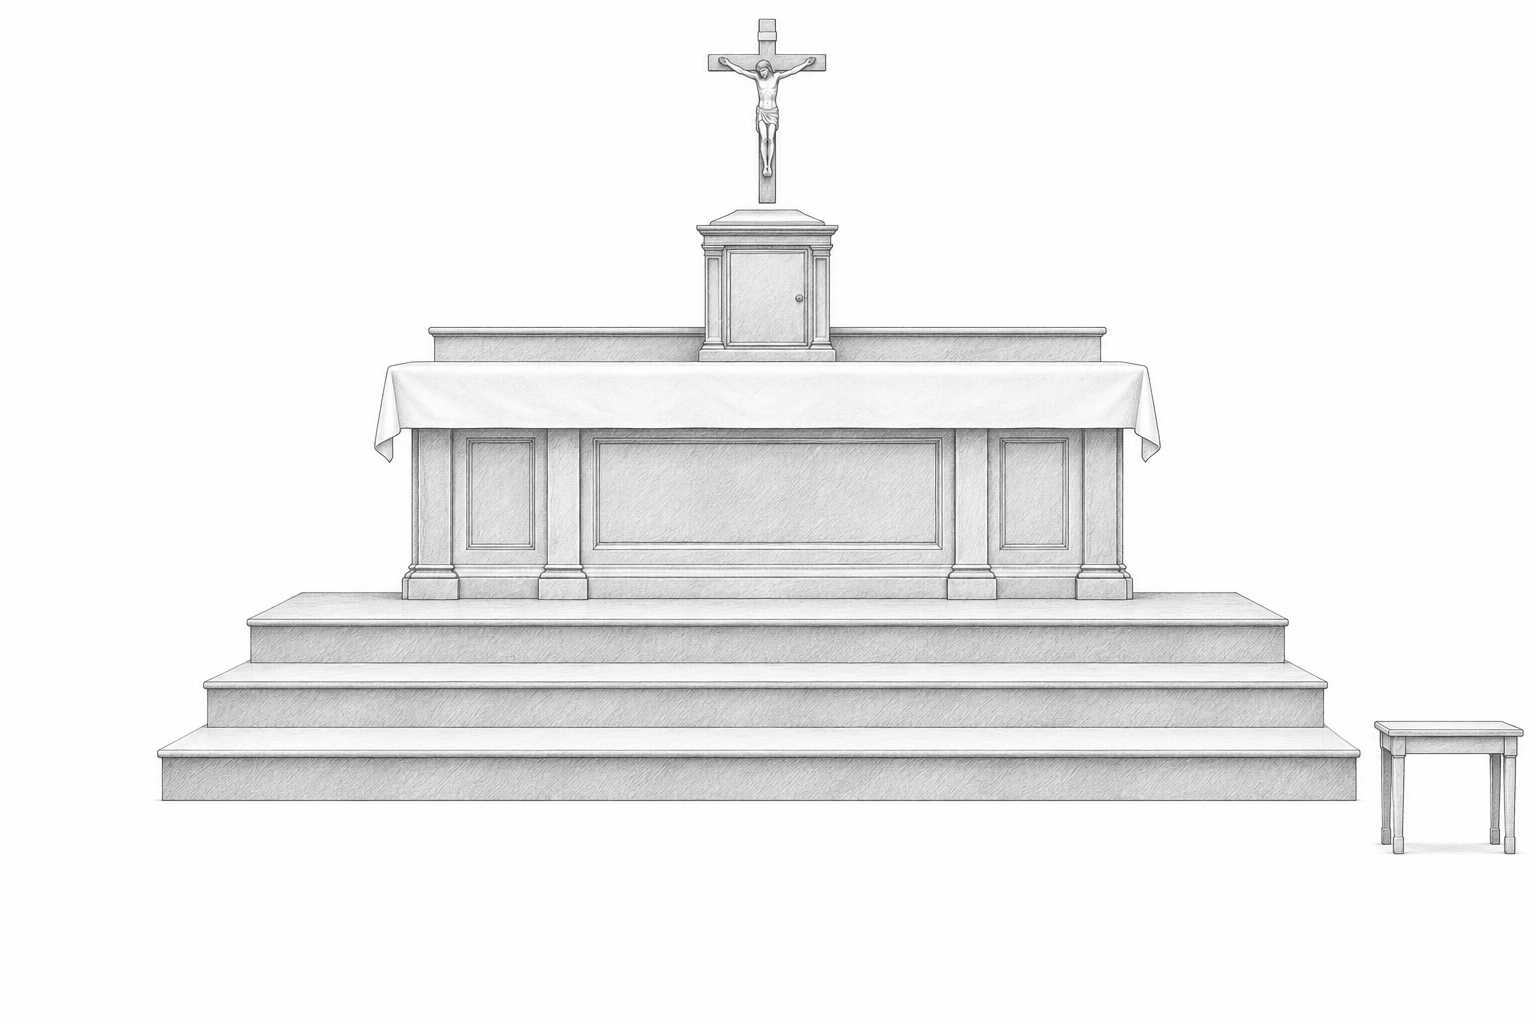
\includegraphics[width=\ASGSceneWidth]{liturgy/roman-rite/1962/reference/altar-server-guides/shared/artwork/pencil/ASG-ART-032-sanctuary-master.png}};
    \node[font=\fontsize{7}{8}\selectfont\bfseries,anchor=north west] at (2,66) {GOSPEL};
    \node[font=\fontsize{7}{8}\selectfont\bfseries,anchor=north east] at (98,66) {EPISTLE};
    \foreach \n/\y in {1/18.3,2/22.5,3/26.5}{%
      \node[asg stop] at (9,\y) {\n};}
    \node[font=\fontsize{6.6}{7.7}\selectfont,anchor=north] at (94,10.8) {CREDENCE};}
\newcommand{\ASGEndScene}{\end{tikzpicture}}

% Save the complete composed sanctuary once. A close view clips that box:
% architecture, appointments, actors and occlusion cannot drift independently.
\newsavebox{\ASGSceneSnapshot}
\newlength{\ASGZoomUnit}
\newcommand{\ASGSaveScene}[2]{%
  \sbox{\ASGSceneSnapshot}{\ASGBeginScene{#1}#2\ASGEndScene}}
\newcommand{\ASGShowSavedScene}{\usebox{\ASGSceneSnapshot}}
\newcommand{\ASGSceneViewport}[5]{%
  \begingroup
  \pgfmathsetlength{\ASGZoomUnit}{#5/(#3-#1)}%
  \begin{tikzpicture}[x=\ASGZoomUnit,y=\ASGZoomUnit]
    \begin{scope}
      \clip (0,0) rectangle (#3-#1,#4-#2);
      \node[anchor=south west,inner sep=0pt] at (-#1,-#2)
        {\resizebox{100\ASGZoomUnit}{!}{\ASGShowSavedScene}};
    \end{scope}
    \pgfresetboundingbox
    \path[use as bounding box] (0,0) rectangle (#3-#1,#4-#2);
    \draw[black!50,line width=.4pt] (0,0) rectangle (#3-#1,#4-#2);
  \end{tikzpicture}%
  \endgroup}

\newcommand{\ASGStandingServer}[3]{%
  \node[anchor=south,inner sep=0pt] at (#1,#2) {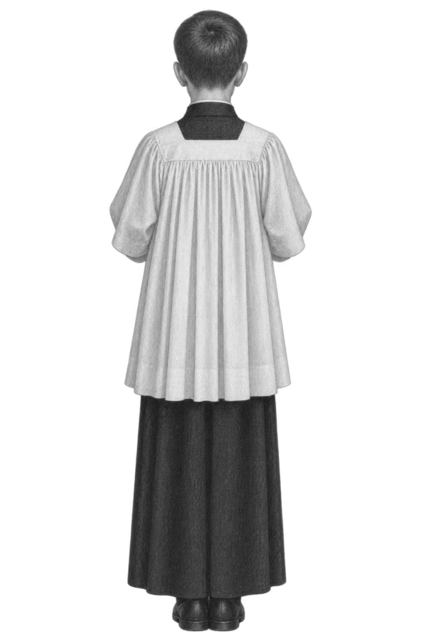
\includegraphics[height=23\ASGSceneUnit]{liturgy/roman-rite/1962/reference/altar-server-guides/shared/artwork/pencil/ASG-ART-033-server-standing.png}};
  \begin{pgfonlayer}{asg labels}\node[asg label,anchor=north] at (#1,#2) {#3};\end{pgfonlayer}}
\newcommand{\ASGKneelingServer}[3]{%
  \node[anchor=south,inner sep=0pt] at (#1,#2) {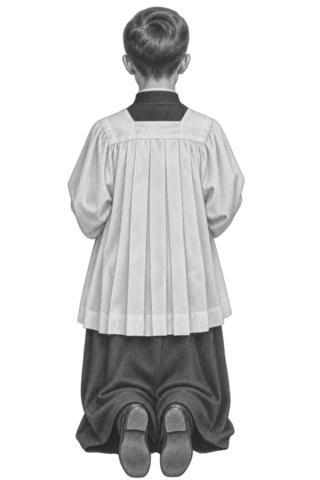
\includegraphics[height=16\ASGSceneUnit]{liturgy/roman-rite/1962/reference/altar-server-guides/shared/artwork/pencil/ASG-ART-034-server-kneeling.png}};
  \begin{pgfonlayer}{asg labels}\node[asg label,anchor=north] at (#1,#2) {#3};\end{pgfonlayer}}
\newcommand{\ASGPriest}[3]{%
  \node[anchor=south,inner sep=0pt] at (#1,#2) {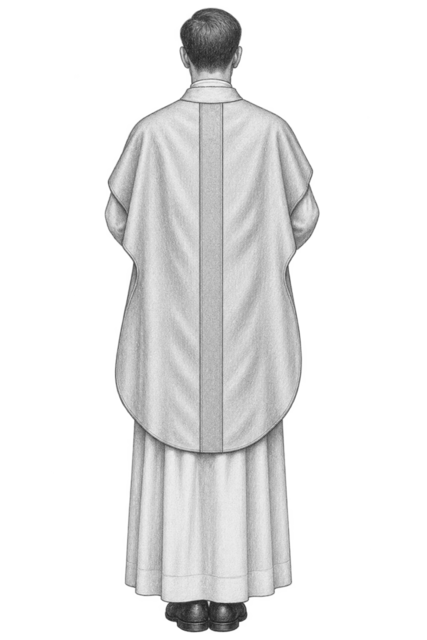
\includegraphics[height=28\ASGSceneUnit]{liturgy/roman-rite/1962/reference/altar-server-guides/shared/artwork/pencil/ASG-ART-035-priest-standing.png}};
  \begin{pgfonlayer}{asg labels}\node[asg label,anchor=north] at (#1,#2) {#3};\end{pgfonlayer}}
\newcommand{\ASGServerFacingLeft}[4][0]{%
  \node[anchor=south,inner sep=0pt] at (#2,#3) {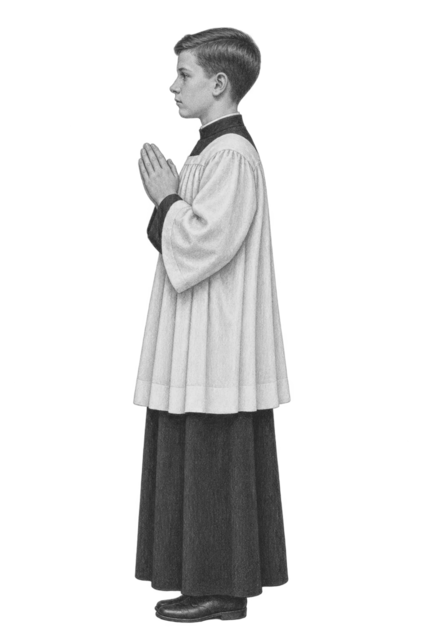
\includegraphics[height=23\ASGSceneUnit]{liturgy/roman-rite/1962/reference/altar-server-guides/shared/artwork/pencil/ASG-ART-037-server-facing-left.png}};
  \begin{pgfonlayer}{asg labels}\node[asg label,anchor=north] at (#2,#3-#1) {#4};\end{pgfonlayer}}
\newcommand{\ASGPriestFacingRight}[3]{%
  \node[anchor=south,inner sep=0pt] at (#1,#2) {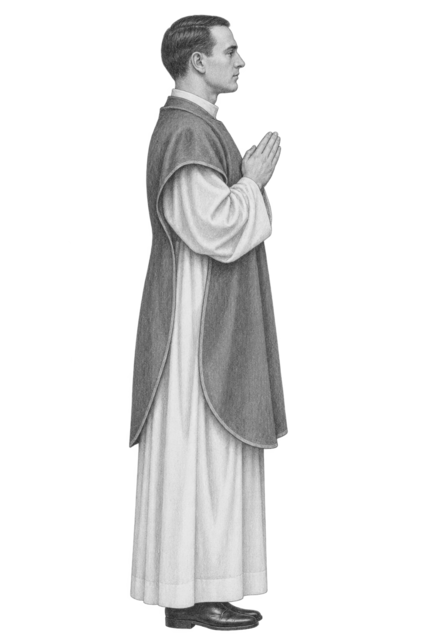
\includegraphics[height=28\ASGSceneUnit]{liturgy/roman-rite/1962/reference/altar-server-guides/shared/artwork/pencil/ASG-ART-038-priest-facing-right.png}};
  \begin{pgfonlayer}{asg labels}\node[asg label,anchor=north] at (#1,#2) {#3};\end{pgfonlayer}}
\newcommand{\ASGCandle}[1]{%
  \node[anchor=south,inner sep=0pt] at (#1,45) {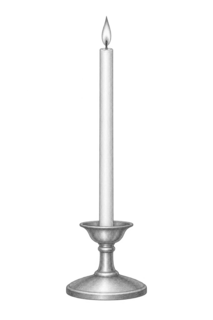
\includegraphics[height=11\ASGSceneUnit]{liturgy/roman-rite/1962/reference/altar-server-guides/shared/artwork/pencil/ASG-ART-036-altar-candle.png}};}
\newcommand{\ASGLowCandles}{\ASGCandle{31}\ASGCandle{69}}
\newcommand{\ASGSungCandles}{%
  \ASGCandle{30}\ASGCandle{36}\ASGCandle{42}%
  \ASGCandle{58}\ASGCandle{64}\ASGCandle{70}}
\newcommand{\ASGStation}[3]{\begin{pgfonlayer}{asg labels}\node[asg label] at (#1,#2) {#3};\end{pgfonlayer}}
\newcommand{\ASGMissalGospel}{\draw[thin] (37,43) -- (37,59);\ASGStation{37}{60}{MISSAL}}
\newcommand{\ASGPairPlan}[2]{%
  \begin{pgfonlayer}{asg labels}
  \filldraw[fill=white,draw=black!60] (12,24) rectangle (43,47);
  \node[font=\fontsize{6.5}{7.5}\selectfont\bfseries] at (27.5,44) {ABOVE: SIDE BY SIDE};
  \node[asg label] at (18,33) {P};
  \node[asg label] at (34,38) {#1};
  \node[asg label] at (34,28) {#2};
  \draw[-{Stealth[length=1.2mm]}] (28,38) -- (22,35);
  \draw[-{Stealth[length=1.2mm]}] (28,28) -- (22,31);
  \end{pgfonlayer}}
\newcommand{\ASGStop}[3]{\node[asg stop] at (#1,#2) {#3};}

\newcommand{\ASGOrientationKey}{%
  \par\smallskip\noindent\textbf{Look from the nave toward the altar.}
  Gospel stays picture-left; Epistle stays picture-right. The same altar,
  three levels and credence remain in every position view: 1 is the lowest
  step, 2 the second step, and 3 the predella. Lettered circles on a dashed
  route are successive stops, not extra people. Figures show the named
  standing or kneeling station; close views teach the hand action.
  The actual distances, reverences and side lanes are rehearsed locally.
  \par\smallskip}

\newcommand{\ASGMovementFields}[5]{%
  \par\smallskip\noindent{\small
  \textbf{Cue:} #1\quad\textbf{Who / object:} #2\par
  \textbf{Route:} #3\par
  \textbf{Finish:} #4\par
  \textbf{Waiting:} #5\par}\smallskip}

% Resting objects for the shared Low Mass sanctuary. Load after
% sanctuary-scenes.tex. Every (x,y) argument is the midpoint of the lowest
% visible support/contact line, in ASGSceneUnit coordinates. These macros
% draw objects only; the calling scene owns labels, routes and occupancy.
% Insets use the existing dictionary files directly, with no asset copies.
% Trims are in bp, matching the source images' 72 dpi coordinate space.
\newcommand{\LMRestingMissalHeight}{5.5\ASGSceneUnit}
\newcommand{\LMRestingBellHeight}{4.0\ASGSceneUnit}
\newcommand{\LMRestingCruetsHeight}{3.3\ASGSceneUnit}
\newcommand{\LMRestingVeilWidth}{7.5\ASGSceneUnit}
\newcommand{\LMCoveredChaliceObjectHeight}{9\ASGSceneUnit}
\newcommand{\LMUncoveredChaliceObjectHeight}{4.0\ASGSceneUnit}
\newcommand{\LMRestingLavaboBasinWidth}{3.4\ASGSceneUnit}
\newcommand{\LMRestingLavaboTowelWidth}{3.4\ASGSceneUnit}
\newcommand{\LMRestingCommunionPlateWidth}{3\ASGSceneUnit}
\newlength{\LMObjectClipHeight}

% Gospel: the reading face turns toward picture-right and the priest.
% Epistle: the book and stand face straight forward. Neither state is made
% by mirroring the other; each retains its own inspected perspective.
\newcommand{\LMMissalObjectGOSPEL}[2]{%
  \node[anchor=south,inner sep=0pt,outer sep=0pt] at (#1,#2) {%
    
\includegraphics[height=\LMRestingMissalHeight,
      trim=90bp 176bp 2bp 287bp,clip]{liturgy/roman-rite/1962/reference/roman-sanctuary-dictionary/shared/artwork/pencil/books/RPD-FIG-books-0001-in-use-missal-on-stand-v3-alpha.png}};}
\newcommand{\LMMissalObjectEPISTLE}[2]{%
  \node[anchor=south,inner sep=0pt,outer sep=0pt] at (#1,#2) {%
    
\includegraphics[height=\LMRestingMissalHeight,
      trim=66bp 46bp 65bp 44bp,clip]{liturgy/roman-rite/1962/reference/altar-server-guides/shared/artwork/pencil/ASG-ART-068-missal-on-stand-straight.png}};}
\newcommand{\LMRestingMissal}[3]{%
  \begingroup
  \edef\LMObjectOrientation{#3}%
  \def\LMGospelOrientation{GOSPEL}%
  \def\LMEpistleOrientation{EPISTLE}%
  \ifx\LMObjectOrientation\LMGospelOrientation
    \LMMissalObjectGOSPEL{#1}{#2}%
  \else
    \ifx\LMObjectOrientation\LMEpistleOrientation
      \LMMissalObjectEPISTLE{#1}{#2}%
    \else
      \PackageError{low-mass-objects}{Unknown Missal orientation #3}{Use GOSPEL or EPISTLE.}%
    \fi
  \fi
  \endgroup}

\newcommand{\LMRestingBell}[2]{%
  \node[anchor=south,inner sep=0pt,outer sep=0pt] at (#1,#2) {%
    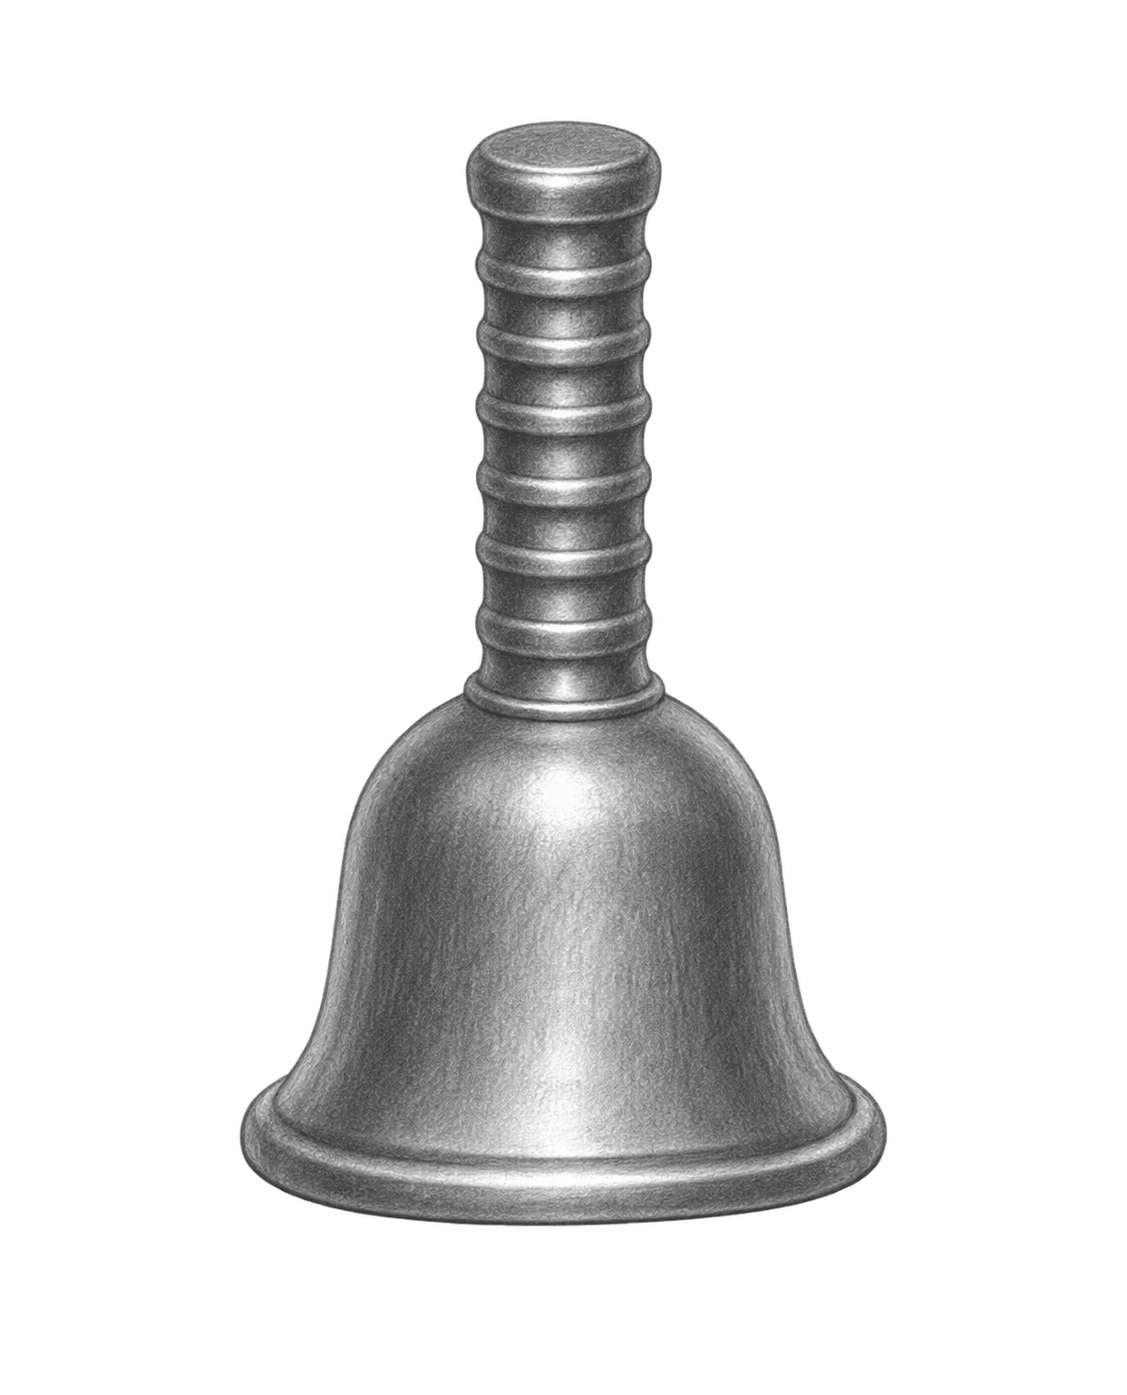
\includegraphics[height=\LMRestingBellHeight,
      trim=239bp 168bp 239bp 120bp,clip]{liturgy/roman-rite/1962/reference/altar-server-guides/shared/artwork/pencil/ASG-ART-063-single-handbell.png}};}

\newcommand{\LMRestingCruets}[2]{%
  \node[anchor=south,inner sep=0pt,outer sep=0pt] at (#1,#2) {%
    
\includegraphics[height=\LMRestingCruetsHeight,
      trim=289bp 164bp 261bp 185bp,clip]{liturgy/roman-rite/1962/reference/roman-sanctuary-dictionary/shared/artwork/pencil/RPD-FIG-service-objects-0103-paired-cruets-v2-alpha.png}};}

% The left member is assigned to wine in this model. Its generic shape does
% not identify its contents. Use this alone while Second carries the water.
\newcommand{\LMRestingWineCruet}[2]{%
  \node[anchor=south,inner sep=0pt,outer sep=0pt] at (#1,#2) {%
    
\includegraphics[height=\LMRestingCruetsHeight,
      trim=289bp 164bp 811bp 185bp,clip]{liturgy/roman-rite/1962/reference/roman-sanctuary-dictionary/shared/artwork/pencil/RPD-FIG-service-objects-0103-paired-cruets-v2-alpha.png}};}

\newcommand{\LMRestingVeil}[2]{%
  \node[anchor=south,inner sep=0pt,outer sep=0pt] at (#1,#2) {%
    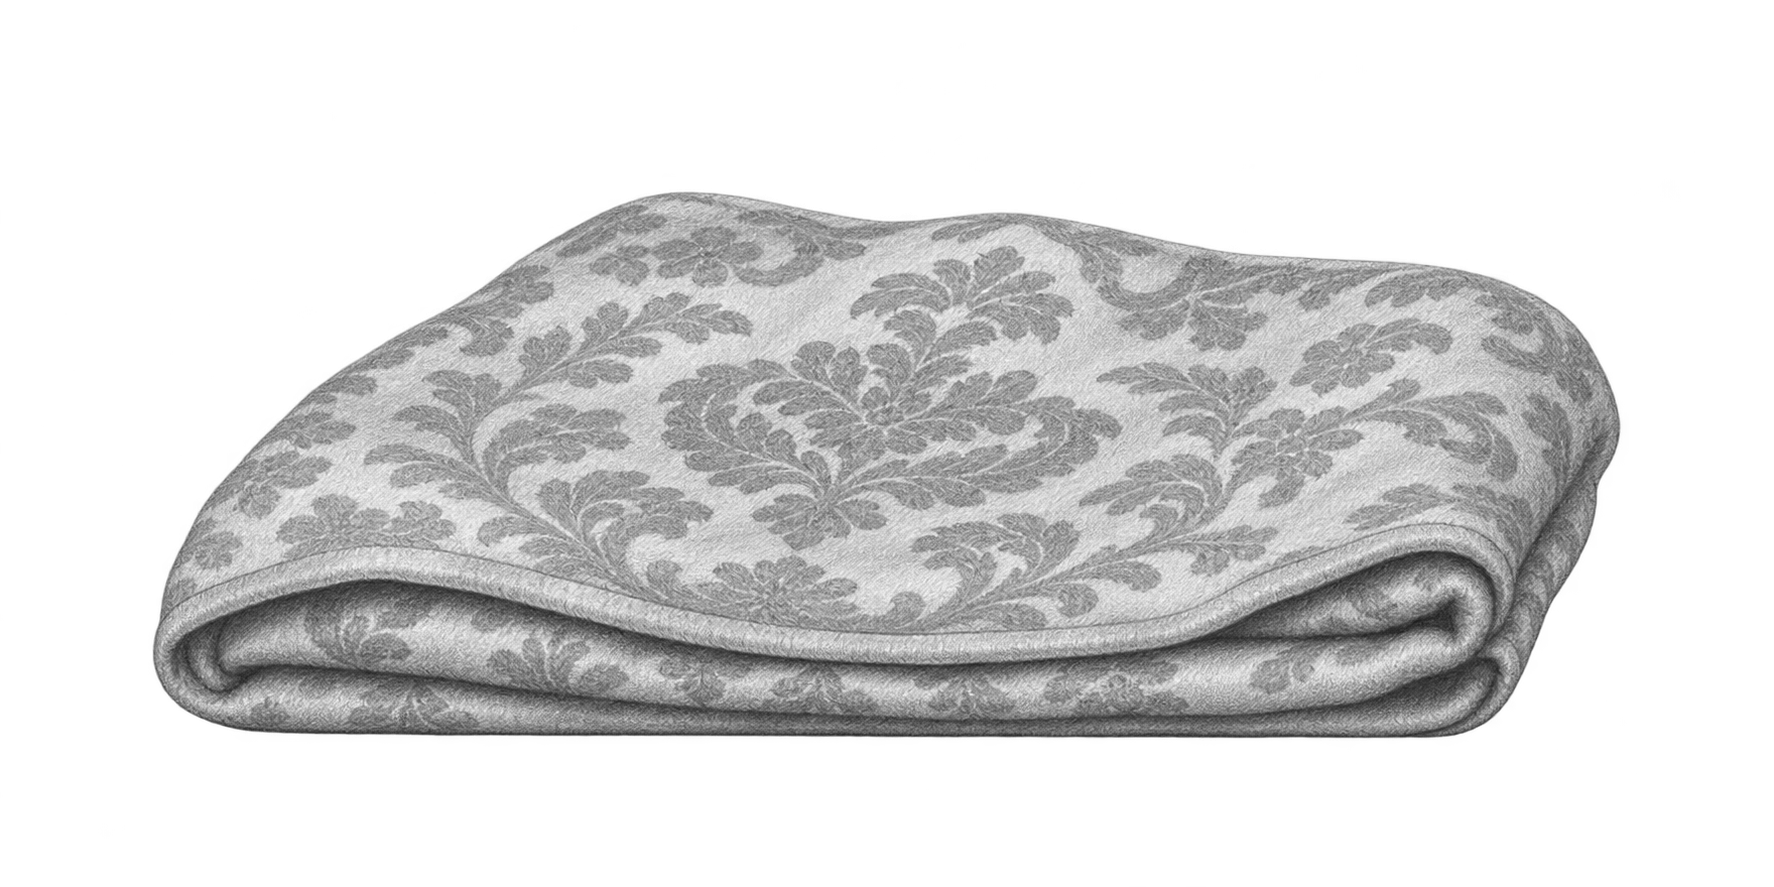
\includegraphics[width=\LMRestingVeilWidth,
      trim=152bp 148bp 153bp 191bp,clip]{liturgy/roman-rite/1962/reference/altar-server-guides/shared/artwork/pencil/ASG-ART-062-folded-chalice-veil.png}};}

% Separate crops of the dictionary's paired basin/manuterge study let the
% caller remove either object when it is being carried. The folded towel
% is the manuterge, not the purificator or folded chalice veil.
\newcommand{\LMRestingLavaboBasin}[2]{%
  \node[anchor=south,inner sep=0pt,outer sep=0pt] at (#1,#2) {%
    
\includegraphics[width=\LMRestingLavaboBasinWidth,
      trim=67bp 253bp 1034bp 323bp,clip]{liturgy/roman-rite/1962/reference/roman-sanctuary-dictionary/shared/artwork/pencil/RPD-FIG-service-objects-0106-lavabo-basin-manuterge-v2-alpha.png}};}
\newcommand{\LMRestingLavaboTowel}[2]{%
  \node[anchor=south,inner sep=0pt,outer sep=0pt] at (#1,#2) {%
    
\includegraphics[width=\LMRestingLavaboTowelWidth,
      trim=803bp 130bp 44bp 177bp,clip]{liturgy/roman-rite/1962/reference/roman-sanctuary-dictionary/shared/artwork/pencil/RPD-FIG-service-objects-0106-lavabo-basin-manuterge-v2-alpha.png}};}

% The distinct Communion plate has the one-wood-handle morphology used in
% the action study. It is not the priest's paten or the lavabo basin.
\newcommand{\LMRestingCommunionPlate}[2]{%
  \node[anchor=south,inner sep=0pt,outer sep=0pt] at (#1,#2) {%
    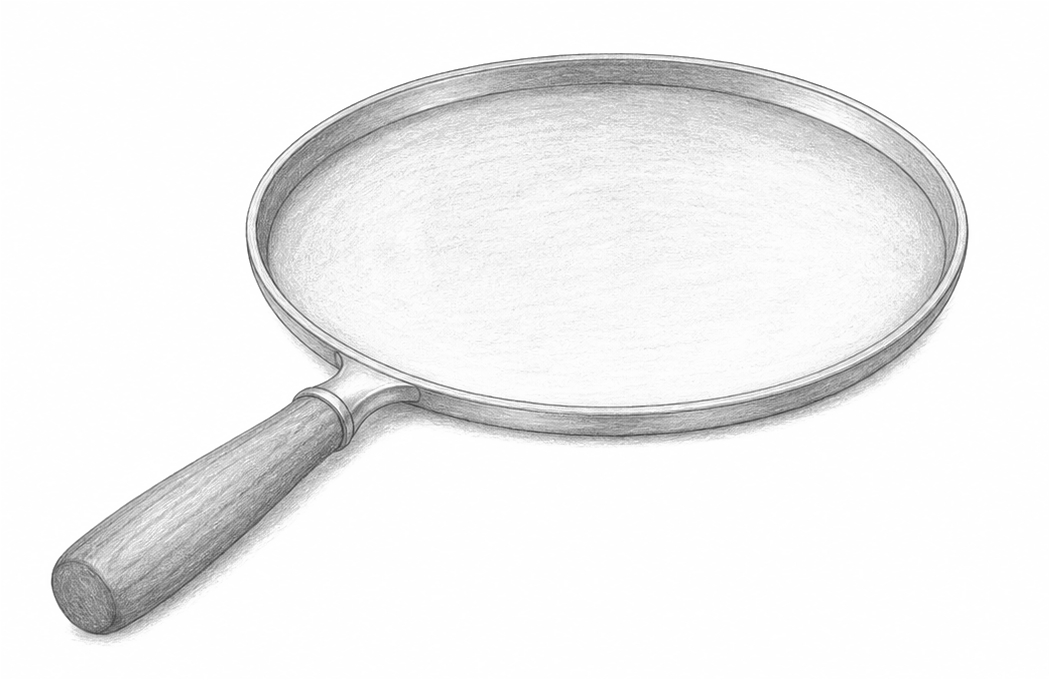
\includegraphics[width=\LMRestingCommunionPlateWidth,
      trim=50bp 44bp 81bp 50bp,clip]{liturgy/roman-rite/1962/reference/roman-sanctuary-dictionary/shared/artwork/pencil/RPD-FIG-sacred-vessels-0007-iso-communion-plate.png}};}

% The isolated round-foot vessel follows the same bowl, node and foot
% shown in the held-chalice and finger-ablution action sprites.
\newcommand{\LMUncoveredChaliceObject}[2]{%
  \node[anchor=south,inner sep=0pt,outer sep=0pt] at (#1,#2) {%
    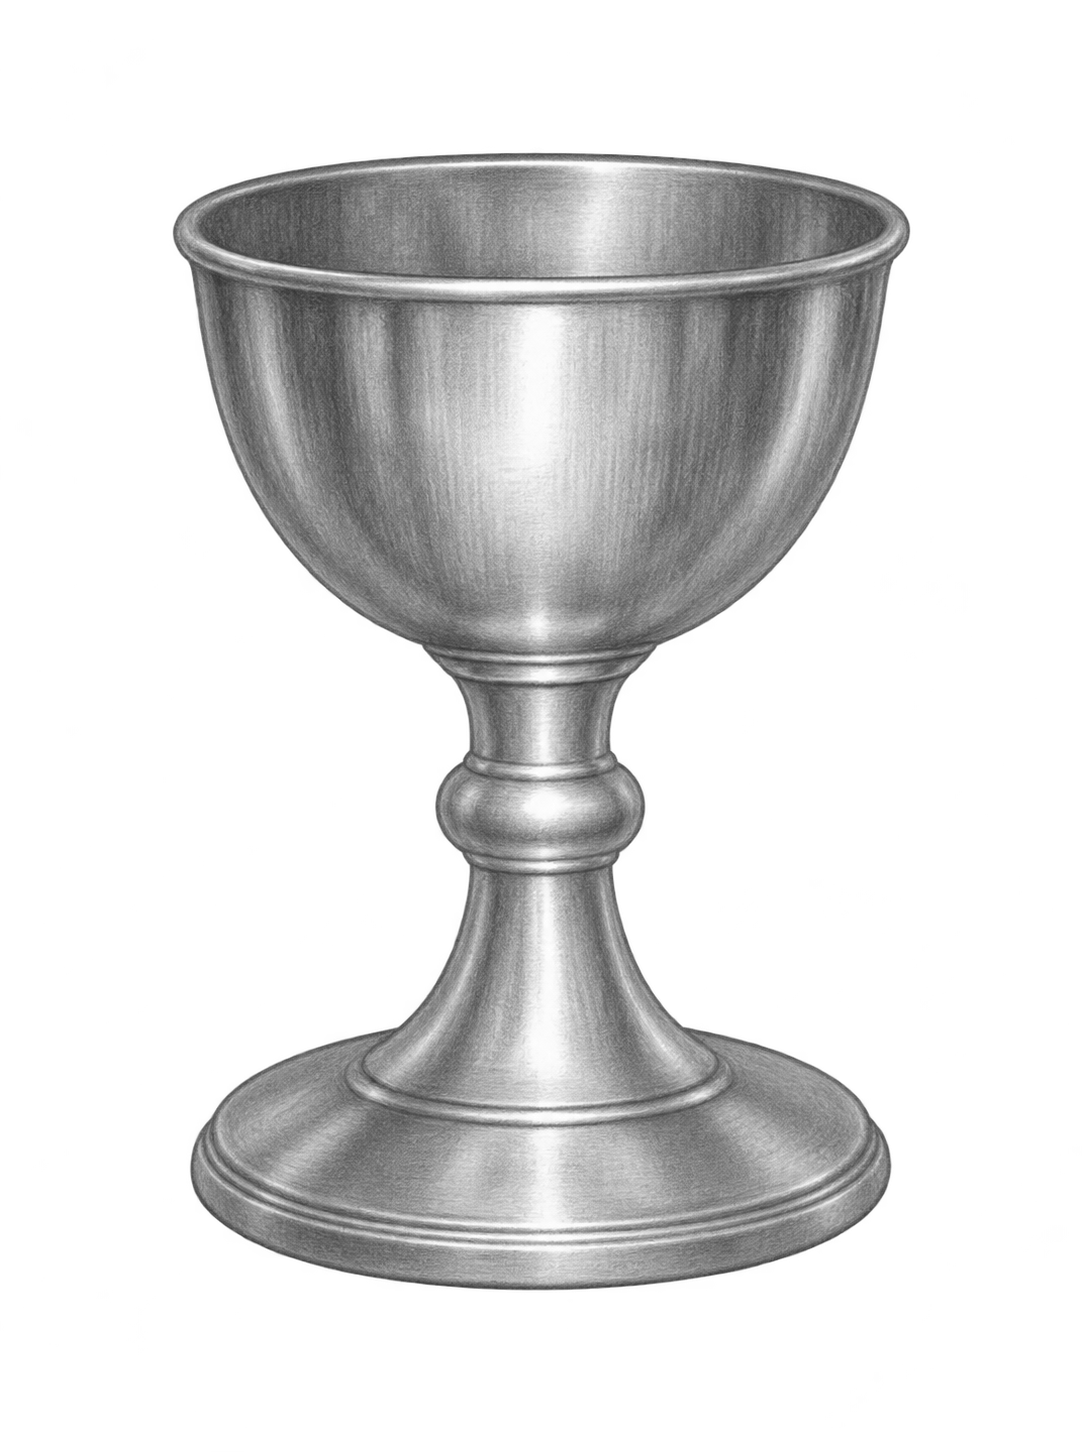
\includegraphics[height=\LMUncoveredChaliceObjectHeight,
      trim=172bp 161bp 172bp 152bp,clip]{liturgy/roman-rite/1962/reference/altar-server-guides/shared/artwork/pencil/ASG-ART-076-uncovered-chalice.png}};}

% After the offering, the pall covers the chalice before the Lavabo.
% The small plain square is a perspective recognition mark, not a claim
% about the pall's construction or dimensions. The vessel base is unchanged.
\newcommand{\LMChaliceWithPallObject}[2]{%
  \begin{scope}[shift={(#1,#2)}]
  \LMUncoveredChaliceObject{0}{0}%
  \setlength{\LMObjectClipHeight}{\LMUncoveredChaliceObjectHeight}%
  \path[fill=white,draw=black!65,line width=.2pt]
    (-.365\LMObjectClipHeight,.86\LMObjectClipHeight) --
    (.335\LMObjectClipHeight,.86\LMObjectClipHeight) --
    (.385\LMObjectClipHeight,1.015\LMObjectClipHeight) --
    (-.315\LMObjectClipHeight,1.015\LMObjectClipHeight) -- cycle;
  \end{scope}}

% Isolate only the already assembled, covered chalice at the left of the
% dictionary's formation study. The stepped clip removes the separate
% corporal in the lower-right corner without cutting the veil above it.
\newcommand{\LMCoveredChaliceObject}[2]{%
  \begin{scope}[shift={(#1,#2)}]
  \setlength{\LMObjectClipHeight}{\LMCoveredChaliceObjectHeight}%
  \clip (-.525\LMObjectClipHeight,0) --
    (.32\LMObjectClipHeight,0) --
    (.32\LMObjectClipHeight,.29\LMObjectClipHeight) --
    (.525\LMObjectClipHeight,.29\LMObjectClipHeight) --
    (.525\LMObjectClipHeight,\LMObjectClipHeight) --
    (-.525\LMObjectClipHeight,\LMObjectClipHeight) -- cycle;
  \node[anchor=south,inner sep=0pt,outer sep=0pt] at (0,0) {%
    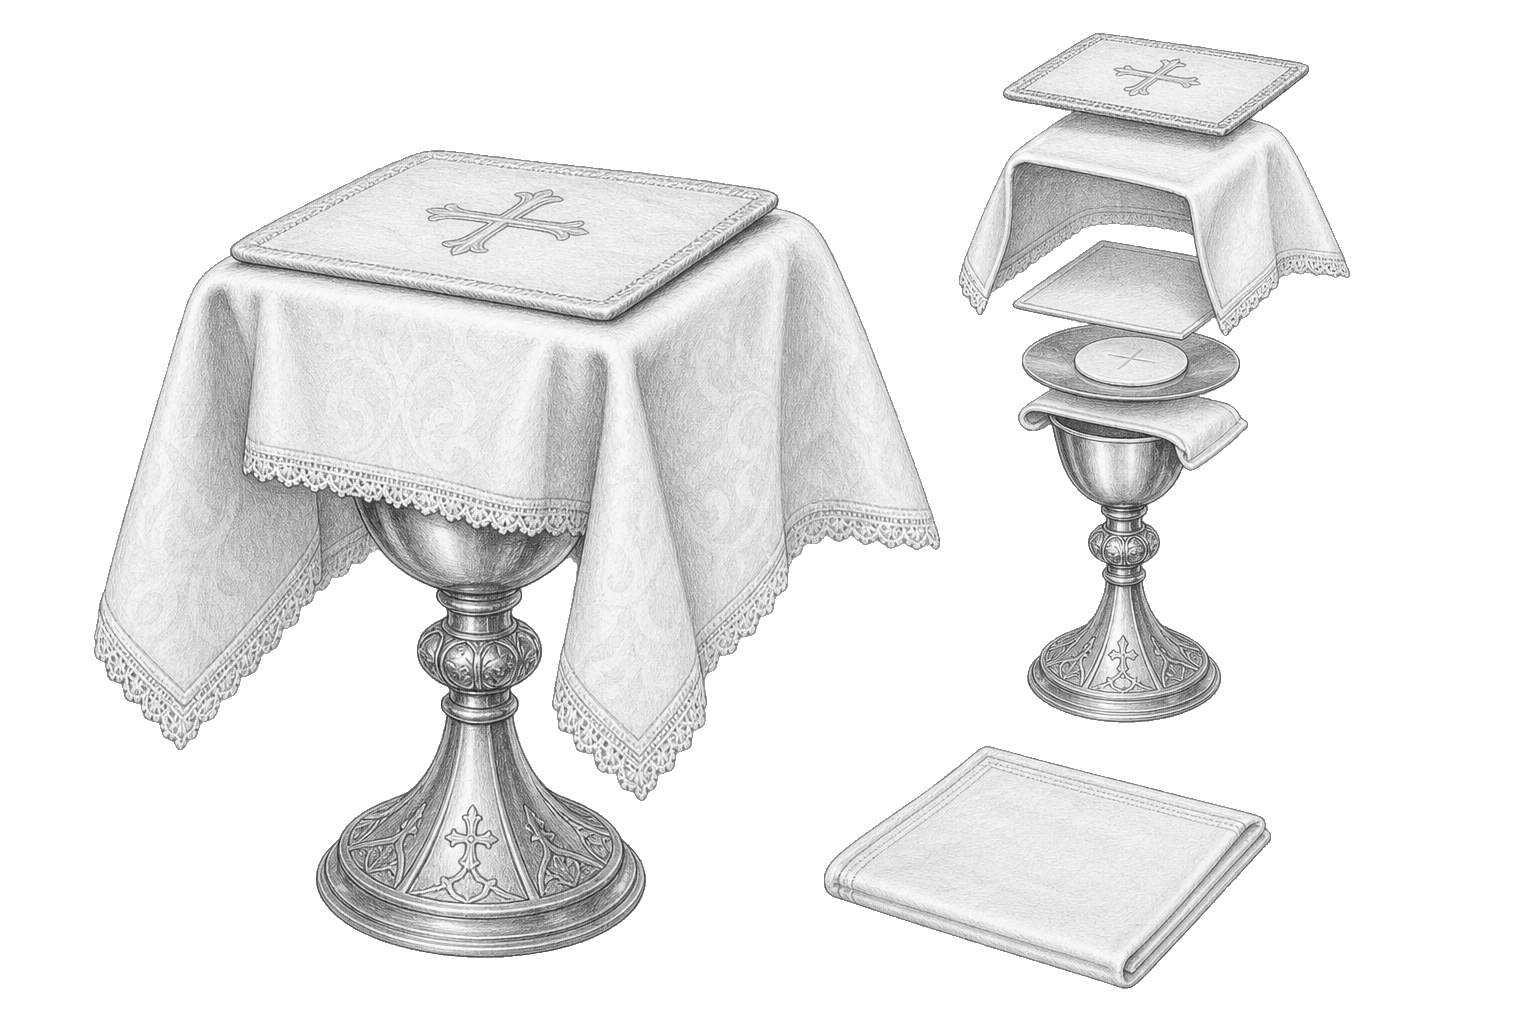
\includegraphics[height=\LMCoveredChaliceObjectHeight,
      trim=94bp 63bp 590bp 149bp,clip]{liturgy/roman-rite/1962/reference/roman-sanctuary-dictionary/shared/artwork/pencil/compositions/RPD-FIG-prepared-chalice-0001-formation-alpha.png}};
  \end{scope}}

\tikzset{lm role tag/.style={asg label},lm object tag/.style={asg label},lm transfer tag/.style={asg label}}
\ifTrainerManualGuide
  \newcommand{\LMPencilSceneHeight}{4.05cm}
  \newcommand{\LMPositionWidth}{9.5cm}
\else
  \newcommand{\LMPencilSceneHeight}{5.00cm}
  \newcommand{\LMPositionWidth}{10.5cm}
\fi
\newcommand{\LMPositionScene}[2]{%
  \ASGSaveScene{\LMPositionWidth}{\ASGLowCandles #1}%
  \par\smallskip\noindent\makebox[\linewidth][c]{\ASGShowSavedScene}%
  \par\noindent{\small\centering #2\par}\smallskip}
% x1,y1,x2,y2 use the same 0--100 sanctuary coordinates as the wide view.
% The backdrop starts at y=0. A viewport changes only crop and magnification.
\newcommand{\LMSceneEnlargement}[6]{%
  \par\smallskip
  \noindent\makebox[\linewidth][c]{%
    \ASGSceneViewport{#1}{#2}{#3}{#4}{#5}}%
  \par{\small\centering\textbf{Detail of the scene above.} #6\par}%
  \smallskip}
\newcommand{\LMRouteFields}[6]{%
  \par\smallskip{\fontsize{10.5}{12.5}\selectfont\RaggedRight
  \textbf{Cue:} #1\quad\textbf{Who / object:} #2\par
  \textbf{Start:} #3\par
  \textbf{Route:} #4\par
  \textbf{Finish / facing:} #5\par
  \textbf{Waiting:} #6\par}\smallskip}
\newcommand{\LMMissalAtEpistle}{\LMRestingMissal{63}{43}{EPISTLE}\ASGStation{63}{51}{MISSAL}}
\newcommand{\LMMissalAtGospel}{\LMRestingMissal{37}{43}{GOSPEL}\ASGStation{37}{58}{MISSAL}}
\newcommand{\LMCoveredChalice}{\LMCoveredChaliceObject{50}{43}\draw[thin] (22,40) -- (48,43);\ASGStation{12}{40}{COVERED\\CHALICE}}
\newcommand{\LMPriestAbove}[2]{%
  \node[anchor=south,inner sep=0pt] at (#1,#2) {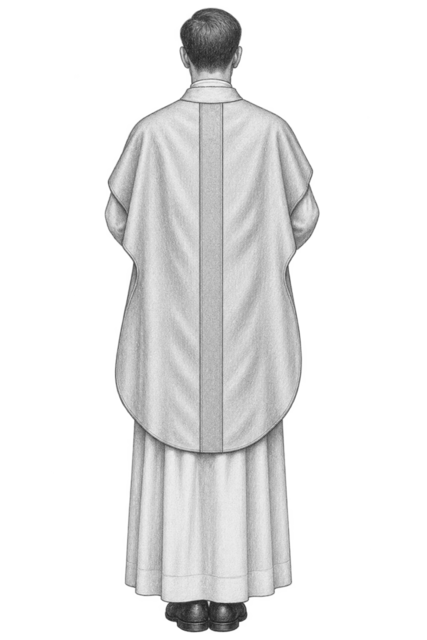
\includegraphics[height=28\ASGSceneUnit]{liturgy/roman-rite/1962/reference/altar-server-guides/shared/artwork/pencil/ASG-ART-035-priest-standing.png}};
  \ASGStation{#1}{#2+31}{PRIEST}}
\newcommand{\LMPriestFacingLeft}[3]{%
  \node[anchor=south,inner sep=0pt] at (#1,#2) {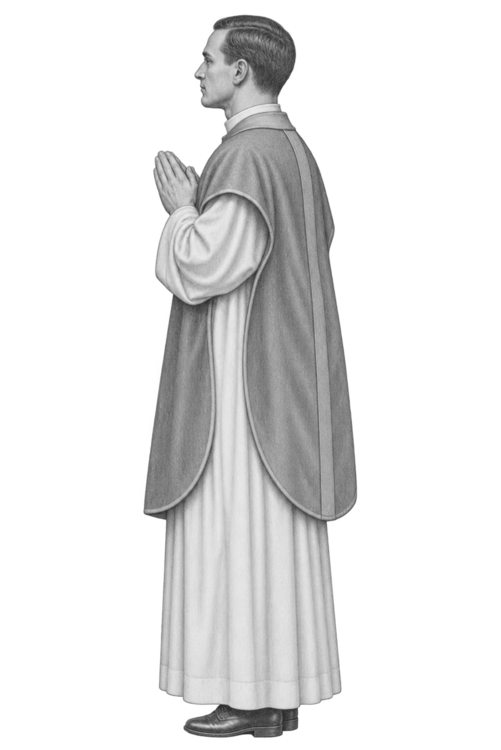
\includegraphics[height=28\ASGSceneUnit,trim=0 7 0 12,clip]{liturgy/roman-rite/1962/reference/altar-server-guides/shared/artwork/pencil/ASG-ART-039-priest-facing-left.png}};
  \ASGStation{#1}{#2-2}{#3}}
\newcommand{\LMBookBearer}[3]{%
  \node[anchor=south,inner sep=0pt] at (#1,#2) {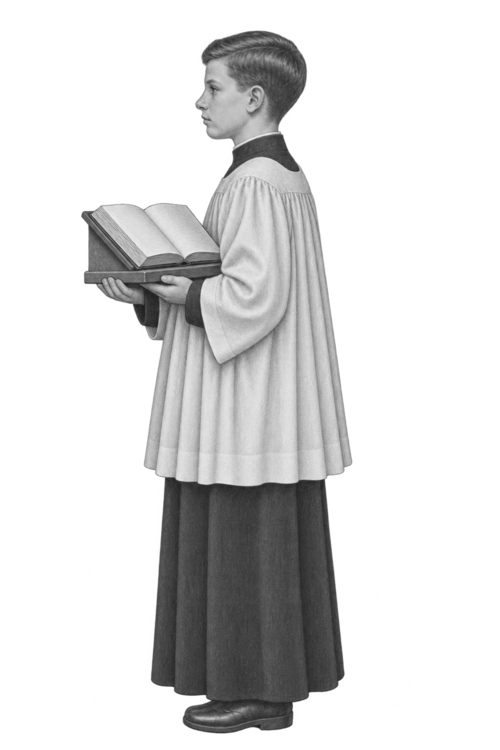
\includegraphics[height=23\ASGSceneUnit,trim=0 13 0 28,clip]{liturgy/roman-rite/1962/reference/altar-server-guides/shared/artwork/pencil/ASG-ART-040-server-carrying-missal.png}};
  \ASGStation{#1}{#2-2}{#3}}
\newcommand{\LMWaitingCruetServer}[4]{%
  \node[anchor=south,inner sep=0pt] at (#1,#2) {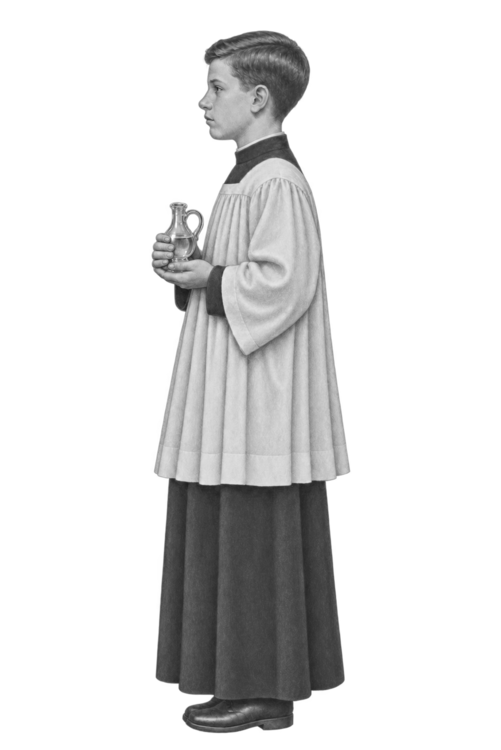
\includegraphics[height=23\ASGSceneUnit,trim=140 15 140 30,clip]{liturgy/roman-rite/1962/reference/altar-server-guides/shared/artwork/pencil/ASG-ART-050-server-waiting-cruet.png}};
  \ASGStation{#1}{#2-#4}{#3}}
\newcommand{\LMCruetKissDetail}{%
  \begin{center}\begin{tikzpicture}
  \node[inner sep=0pt] (art) {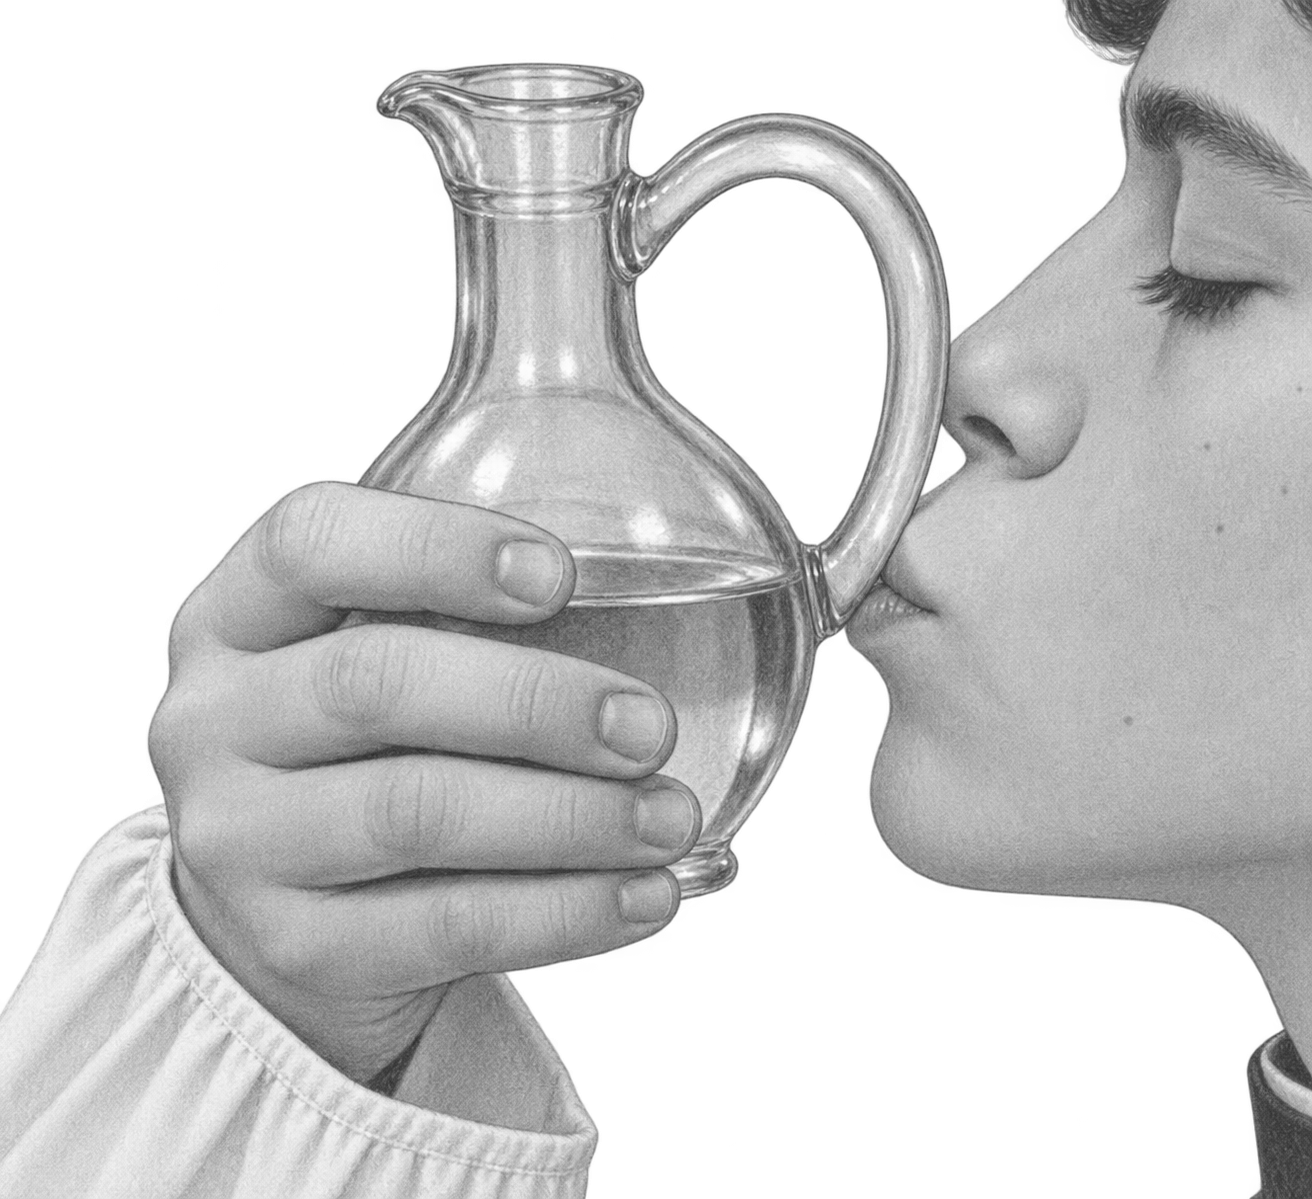
\includegraphics[height=3.2cm]{liturgy/roman-rite/1962/reference/altar-server-guides/shared/artwork/pencil/ASG-ART-041-cruet-kiss.png}};
  \node[asg label,anchor=east] (label) at ($(art.north west)+(-2mm,-4mm)$) {BASE OF\\HANDLE};
  \draw[thin,-{Stealth[length=1.4mm]}] (label.south east) -- ($(art.south west)!.67!(art.south east)+(0,1.55cm)$);
  \end{tikzpicture}\par{\small Kiss the lower handle attachment lightly; keep the spout clear.}\end{center}}

\newcommand{\LMSceneStart}{%
  \LMPositionScene{%
    \LMRestingLavaboTowel{93.6}{19.6}\LMRestingLavaboBasin{93.6}{19.2}
    \LMRestingCommunionPlate{91}{19.2}
    \LMMissalAtEpistle
    \LMChaliceBearer{50}{11.3}{PRIEST}
    \ASGStandingServer{33}{11.3}{SECOND}
    \ASGStandingServer{67}{11.3}{FIRST}
  }{1. Servers form at the foot; the priest arrives carrying the covered chalice, then faces the altar.}}
\newcommand{\LMScenePriestPrepares}{%
  \LMPositionScene{%
    \LMRestingLavaboTowel{93.6}{19.6}\LMRestingLavaboBasin{93.6}{19.2}
    \LMRestingCommunionPlate{91}{19.2}
    \LMRestingCruets{97.2}{19.6}
    \LMMissalAtEpistle\LMCoveredChalice
    \ASGPriest{50}{26.5}{PRIEST}
    \ASGStandingServer{33}{11.3}{SECOND}
    \ASGStandingServer{67}{11.3}{FIRST}
  }{While the priest prepares the altar: both servers remain standing on the floor.}}
\newcommand{\LMSceneFootKneel}{%
  \LMPositionScene{%
    \LMRestingLavaboTowel{93.6}{19.6}\LMRestingLavaboBasin{93.6}{19.2}
    \LMRestingCommunionPlate{91}{19.2}
    \LMRestingCruets{97.2}{19.6}
    \LMMissalAtEpistle\LMCoveredChalice
    \ASGPriest{50}{11.3}{PRIEST}
    \ASGKneelingServer{33}{11.3}{SECOND}
    \ASGKneelingServer{67}{11.3}{FIRST}
  }{2. At the opening prayers: both servers kneel on the floor.}}
\newcommand{\LMSceneRiseFromFoot}{%
  \LMPositionScene{%
    \LMRestingLavaboTowel{93.6}{19.6}\LMRestingLavaboBasin{93.6}{19.2}
    \LMRestingCommunionPlate{91}{19.2}
    \LMRestingCruets{97.2}{19.6}
    \LMMissalAtEpistle\LMCoveredChalice
    \ASGPriest{50}{26.5}{PRIEST}
    \ASGStandingServer{33}{11.3}{SECOND}
    \ASGStandingServer{67}{11.3}{FIRST}
    \draw[asg route] (30,10) -- (23,10) -- (23,17);
    \draw[asg route] (70,10) -- (77,10) -- (77,17);
  }{After the priest starts up: both rise, turn inward, and go to the outside places.}}
\newcommand{\LMSceneNormalPlaces}{%
  \LMPositionScene{%
    \LMRestingLavaboTowel{93.6}{19.6}\LMRestingLavaboBasin{93.6}{19.2}
    \LMRestingCommunionPlate{91}{19.2}
    \LMRestingCruets{97.2}{19.6}
    \LMCoveredChaliceObject{50}{43}
    \LMMissalAtEpistle
    \ASGPriest{50}{26.5}{PRIEST}
    \ASGKneelingServer{25}{18.3}{SECOND}
    \ASGKneelingServer{75}{18.3}{FIRST}
    \draw[asg route] (33,12) -- (25,12) -- (25,17);
    \draw[asg route] (67,12) -- (75,12) -- (75,17);
  }{Movement finished: both kneel at their normal places on Step 1.}}
\newcommand{\LMSceneMissalMove}{%
  \LMPositionScene{%
    \LMRestingLavaboTowel{93.6}{19.6}\LMRestingLavaboBasin{93.6}{19.2}
    \LMRestingCommunionPlate{91}{19.2}
    \ASGPriest{50}{26.5}{PRIEST}
    \ASGStandingServer{20}{11.3}{SECOND\\STAYS}
    \LMBookBearer{72}{26.5}{FIRST}
    \draw[asg route] (73,25) -- (82,18) -- (82,9) -- (50,9);
    \draw[asg route] (48,9) -- (28,9) -- (28,22) -- (35,25);
    \ASGStop{82}{9}{A}\ASGStop{50}{9}{B}\ASGStop{28}{22}{C}
  }{1. First takes the book down the Epistle side; B marks the centre stop.}}
\newcommand{\LMSceneMissalCentre}{%
  \LMPositionScene{%
    \LMRestingLavaboTowel{93.6}{19.6}\LMRestingLavaboBasin{93.6}{19.2}
    \LMRestingCommunionPlate{91}{19.2}
    \LMPriestAbove{50}{26.5}
    \ASGStandingServer{20}{11.3}{SECOND\\STAYS}
    \LMBookBearer{50}{11.3}{FIRST}
    \draw[asg route] (44,10) -- (28,10) -- (28,22) -- (35,25);
    \ASGStop{28}{22}{C}
  }{2. First stops at the centre for the taught reverence, then takes the book up Gospel.}}
\newcommand{\LMSceneGospel}{%
  \LMPositionScene{%
    \LMRestingLavaboTowel{93.6}{19.6}\LMRestingLavaboBasin{93.6}{19.2}
    \LMRestingCommunionPlate{91}{19.2}
    \LMRestingCruets{97.2}{19.6}
    \LMCoveredChaliceObject{50}{43}
    \LMMissalAtGospel
    \LMPriestFacingLeft{39}{26.5}{PRIEST}
    \ASGStandingServer{20}{11.3}{SECOND\\STAYS}
    \ASGStandingServer{29}{22.5}{FIRST}
  }{Gospel begins: First waits at Gospel on Step 2; Second stays below the steps.}}
\newcommand{\LMSceneGospelReturn}{%
  \LMPositionScene{%
    \LMRestingLavaboTowel{93.6}{19.6}\LMRestingLavaboBasin{93.6}{19.2}
    \LMRestingCommunionPlate{91}{19.2}
    \LMMissalAtGospel\LMPriestFacingLeft{39}{26.5}{PRIEST}
    \ASGStandingServer{20}{11.3}{SECOND\\STAYS}
    \ASGServerFacingLeft{75}{11.3}{FIRST}
    \draw[asg route] (29,22) -- (29,6) -- (50,6) -- (75,6) -- (75,10);
    \ASGStop{29}{22}{A}\ASGStop{50}{6}{B}
  }{4. Reading underway: First has descended and returned to Epistle; both face the Gospel.}}
\newcommand{\LMSceneCruetPickup}{%
  \LMPositionScene{%
    \LMRestingLavaboTowel{93.6}{19.6}\LMRestingLavaboBasin{93.6}{19.2}
    \LMRestingCommunionPlate{91}{19.2}
    \LMUncoveredChaliceObject{60}{43}
    \LMMissalAtGospel\ASGPriest{50}{26.5}{PRIEST}
    \ASGStandingServer{71}{11.3}{FIRST}
    \ASGStandingServer{83}{11.3}{SECOND}
    \ASGStation{72}{3}{FIRST: WINE\quad SECOND: WATER}
    \draw[asg route] (25,17) -- (25,6) -- (49,6) -- (75,6) -- (81,10);
    \draw[asg route] (75,17) -- (70,12) -- (52,6);
    \ASGStop{50}{6}{A}
  }{Before pickup: both stand at the credence; the folded veil is already secure.}}
\newcommand{\LMSceneVeilReceipt}{%
  \LMPositionScene{%
    \LMRestingLavaboTowel{93.6}{19.6}\LMRestingLavaboBasin{93.6}{19.2}
    \LMRestingCommunionPlate{91}{19.2}
    \LMUncoveredChaliceObject{60}{43}
    \LMRestingCruets{97.2}{19.6}
    \LMMissalAtGospel\ASGPriest{50}{26.5}{PRIEST}
    \ASGStandingServer{25}{11.3}{SECOND\\WAITS}
    \LMVeilBearer{73}{26.5}{FIRST}
    \draw[asg route] (76,12) -- (82,18) -- (80,24);
  }{After First receives the folded veil at Epistle: Second is still below the steps.}}
\newcommand{\LMSceneBell}{%
  \LMPositionScene{%
    \LMRestingLavaboTowel{93.6}{19.6}\LMRestingLavaboBasin{93.6}{19.2}
    \LMRestingCommunionPlate{91}{19.2}
    \LMChaliceWithPallObject{50}{43}
    \LMRestingCruets{97.2}{19.6}
    \LMMissalAtGospel\LMRestingVeil{70}{43}\ASGPriest{50}{26.5}{PRIEST}
    \ASGKneelingServer{25}{18.3}{SECOND}
    \ASGKneelingServer{75}{18.3}{FIRST}
    \LMRestingBell{80}{22.5}\ASGStation{87}{24}{BELL}
  }{Both kneel on Step 1; the bell rests on Step 2 in front of First.}}
\newcommand{\LMSceneLavaboReset}{%
  \LMPositionScene{%
    \LMRestingLavaboTowel{93.6}{19.6}\LMRestingLavaboBasin{93.6}{19.2}
    \LMRestingCommunionPlate{91}{19.2}
    \LMChaliceWithPallObject{50}{43}
    \LMMissalAtGospel\ASGPriest{50}{26.5}{PRIEST}
    \ASGStandingServer{71}{11.3}{FIRST}
    \ASGStandingServer{83}{11.3}{SECOND}
    \ASGStation{70}{3}{ARTICLES RESET}
    \draw[asg route] (70,10) -- (50,6);
    \ASGStop{50}{6}{A}
  }{1. Lavabo complete: articles are back at the credence; First is ready to take the bell.}}
\newcommand{\LMScenePlatePickup}{%
  \LMPositionScene{%
    \LMRestingLavaboTowel{93.6}{19.6}\LMRestingLavaboBasin{93.6}{19.2}
    \LMRestingCommunionPlate{91}{19.2}
    \LMRestingCruets{97.2}{19.6}\LMRestingBell{80}{22.5}\LMRestingVeil{70}{43}
    \LMMissalAtGospel\ASGPriest{50}{26.5}{PRIEST}
    \ASGKneelingServer{25}{18.3}{SECOND\\WAITS}
    \ASGStandingServer{83}{11.3}{FIRST}
    \ASGStation{66}{4}{BELL SET DOWN; PLATE NEXT}
    \draw[asg route] (75,18) -- (78,13) -- (81,11);
  }{Before the Communion-plate pickup: First is at the credence; Second stays at Gospel.}}
\newcommand{\LMSceneAblutionPickup}{%
  \LMPositionScene{%
    \LMRestingLavaboTowel{93.6}{19.6}\LMRestingLavaboBasin{93.6}{19.2}
    \LMMissalAtGospel\ASGPriest{50}{26.5}{PRIEST}
    \ASGStandingServer{25}{11.3}{SECOND\\WAITS}
    \ASGStandingServer{83}{11.3}{FIRST}
    \ASGStation{66}{4}{FIRST TAKES WINE + WATER}
    \draw[asg route] (88,12) -- (88,19) -- (79,22);
  }{Before pickup: First takes both cruets; Second remains below the Gospel-side steps.}}
\newcommand{\LMSceneElevationReturn}{%
  \LMPositionScene{%
    \LMRestingLavaboTowel{93.6}{19.6}\LMRestingLavaboBasin{93.6}{19.2}
    \LMRestingCommunionPlate{91}{19.2}
    \LMChaliceWithPallObject{50}{43}
    \LMRestingCruets{97.2}{19.6}\LMRestingVeil{70}{43}
    \LMMissalAtGospel\ASGPriest{50}{26.5}{PRIEST}
    \ASGKneelingServer{25}{18.3}{SECOND}
    \ASGKneelingServer{75}{18.3}{FIRST}
    \LMRestingBell{80}{22.5}\ASGStation{87}{24}{BELL}
  }{Return complete: both kneel at the normal places; First has replaced the bell on Step 2.}}
\newcommand{\LMSceneBookReturn}{%
  \LMPositionScene{%
    \LMRestingLavaboTowel{93.6}{19.6}\LMRestingLavaboBasin{93.6}{19.2}
    \LMRestingCommunionPlate{91}{19.2}
    \LMUncoveredChaliceObject{44}{43}
    \ASGPriest{50}{26.5}{PRIEST}
    \LMBookBearer{29}{26.5}{SECOND}
    \LMVeilBearer{72}{22.5}{FIRST}
    \draw[asg route] (29,23) -- (29,9) -- (76,9) -- (76,25);
    \draw[asg route] (72,20) -- (67,5) -- (22,5) -- (22,23);
    \ASGStation{45}{16}{BOOK TO EPISTLE}
    \ASGStop{68.3}{9}{A}
    \ASGStation{82}{58}{FIRST WAITS\\UNTIL A IS CLEAR}
    \ASGStation{46}{2}{FOLDED VEIL TO GOSPEL}
  }{1. Two routes: First gives way while Second passes the crossing A.}}
\newcommand{\LMSceneBookReturnComplete}{%
  \LMPositionScene{%
    \LMRestingLavaboTowel{93.6}{19.6}\LMRestingLavaboBasin{93.6}{19.2}
    \LMRestingCommunionPlate{91}{19.2}
    \LMUncoveredChaliceObject{44}{43}
    \LMRestingCruets{97.2}{19.6}\LMRestingBell{80}{22.5}
    \LMMissalAtEpistle\ASGPriest{50}{26.5}{PRIEST}
    \LMRestingVeil{31}{43}\ASGStation{31}{49}{FOLDED VEIL}
    \ASGKneelingServer{25}{18.3}{SECOND}
    \ASGKneelingServer{75}{18.3}{FIRST}
  }{Objects placed and centre reverence complete: both kneel at their normal places.}}
\newcommand{\LMSceneLastGospel}{%
  \LMPositionScene{%
    \LMRestingLavaboTowel{93.6}{19.6}\LMRestingLavaboBasin{93.6}{19.2}
    \LMRestingCommunionPlate{91}{19.2}
    \LMRestingCruets{97.2}{19.6}\LMRestingBell{80}{22.5}
    \LMMissalAtEpistle\LMCoveredChalice
    \LMPriestFacingLeft{38}{26.5}{PRIEST}
    \ASGStation{12}{49}{GOSPEL CARD}
    \draw[thin] (22,48) -- (34,43);
    \ASGStandingServer{25}{11.3}{SECOND}
    \ASGServerFacingLeft{75}{11.3}{FIRST}
    \draw[asg route,solid] (68,31) -- (47,34);
  }{Last Gospel: the priest faces left; Second faces the altar and First turns toward him.}}
\newcommand{\LMSceneExit}{%
  \LMPositionScene{%
    \LMRestingLavaboTowel{93.6}{19.6}\LMRestingLavaboBasin{93.6}{19.2}
    \LMRestingCommunionPlate{91}{19.2}
    \LMMissalAtEpistle\LMCoveredChalice
    \ASGPriest{50}{26.5}{PRIEST}
    \ASGStandingServer{33}{11.3}{SECOND}
    \ASGStandingServer{67}{11.3}{FIRST}
  }{1. Both servers have reached the foot; the priest is ready to take his covered chalice.}}
\newcommand{\LMSceneRecess}{%
  \LMPositionScene{%
    \LMRestingLavaboTowel{93.6}{19.6}\LMRestingLavaboBasin{93.6}{19.2}
    \LMRestingCommunionPlate{91}{19.2}
    \LMRestingCruets{97.2}{19.6}\LMRestingBell{80}{22.5}
    \LMMissalAtEpistle
    \ASGServerFacingLeft{15}{11.3}{FIRST}
    \ASGServerFacingLeft{27}{11.3}{SECOND}
    \LMChaliceBearer{44}{11.3}{PRIEST}
    \draw[asg route] (58,3) -- (14,3);
  }{The line advances toward the sacristy: First leads, Second follows, then the priest carrying the chalice.}}

\newcommand{\LMScenePlate}{%
  \LMPositionScene{%
    \LMRestingLavaboTowel{93.6}{19.6}\LMRestingLavaboBasin{93.6}{19.2}
    \LMRestingCruets{97.2}{19.6}\LMRestingBell{80}{22.5}
    \LMMissalAtGospel\LMRestingVeil{70}{43}\LMUncoveredChaliceObject{50}{43}
    \ASGKneelingServer{25}{18.3}{SECOND\\WAITS}
    \node[anchor=south west,inner sep=0pt] at (41.1485,8.6979)
      {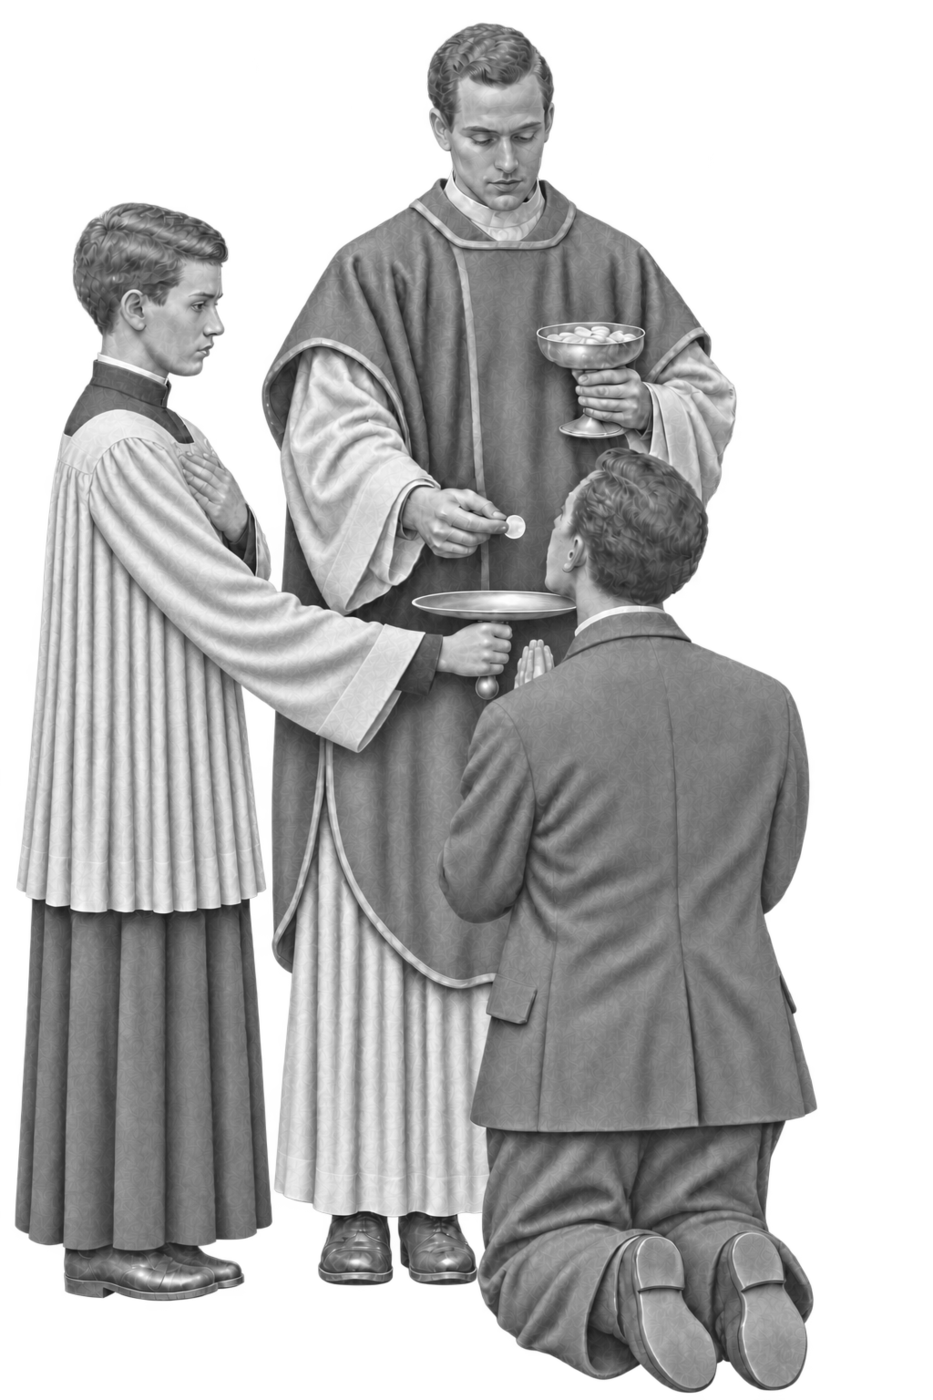
\includegraphics[height=31.1358\ASGSceneUnit]{liturgy/roman-rite/1962/reference/altar-server-guides/shared/artwork/pencil/ASG-ART-078-communion-service-group.png}};
    \ASGStation{40}{8}{FIRST}\ASGStation{51}{5}{PRIEST}
  }{First serves at the priest's right, picture-left; Second remains at Gospel.}%
  \LMSceneEnlargement{46}{24}{61}{33}{6.2cm}{Keep the plate level below the chin, without touching it.}}

% These layers are placed only in the full sanctuary composition. The detail
% below each action clips ASGSceneSnapshot, never an isolated actor layer.
\newcommand{\LMCruetPresentationArt}[1]{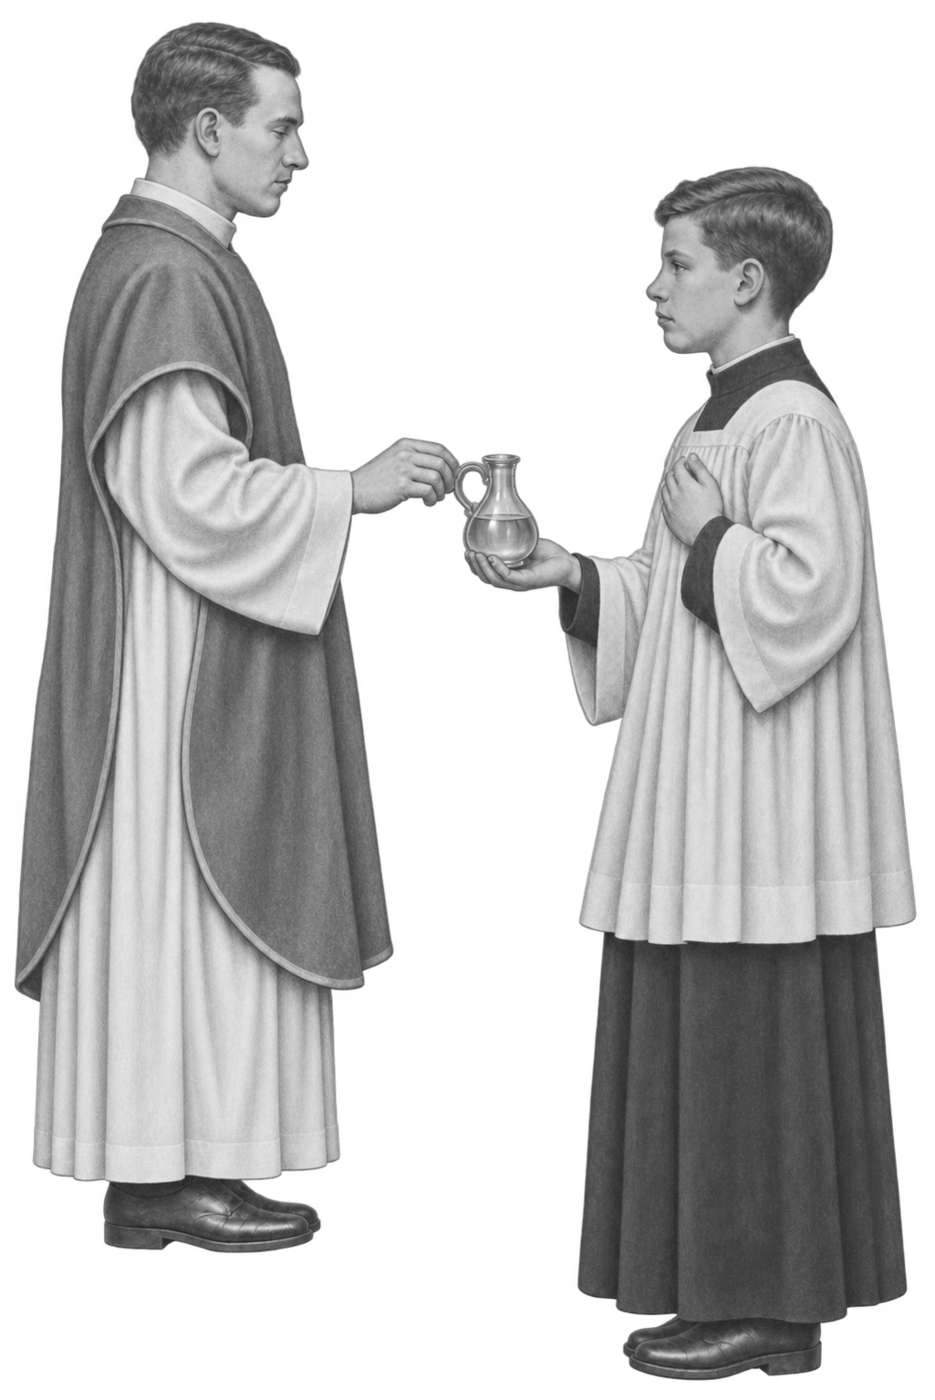
\includegraphics[#1]{liturgy/roman-rite/1962/reference/altar-server-guides/shared/artwork/pencil/ASG-ART-042-cruet-presentation-handle-out.png}}
\newcommand{\LMWinePurificationArt}[1]{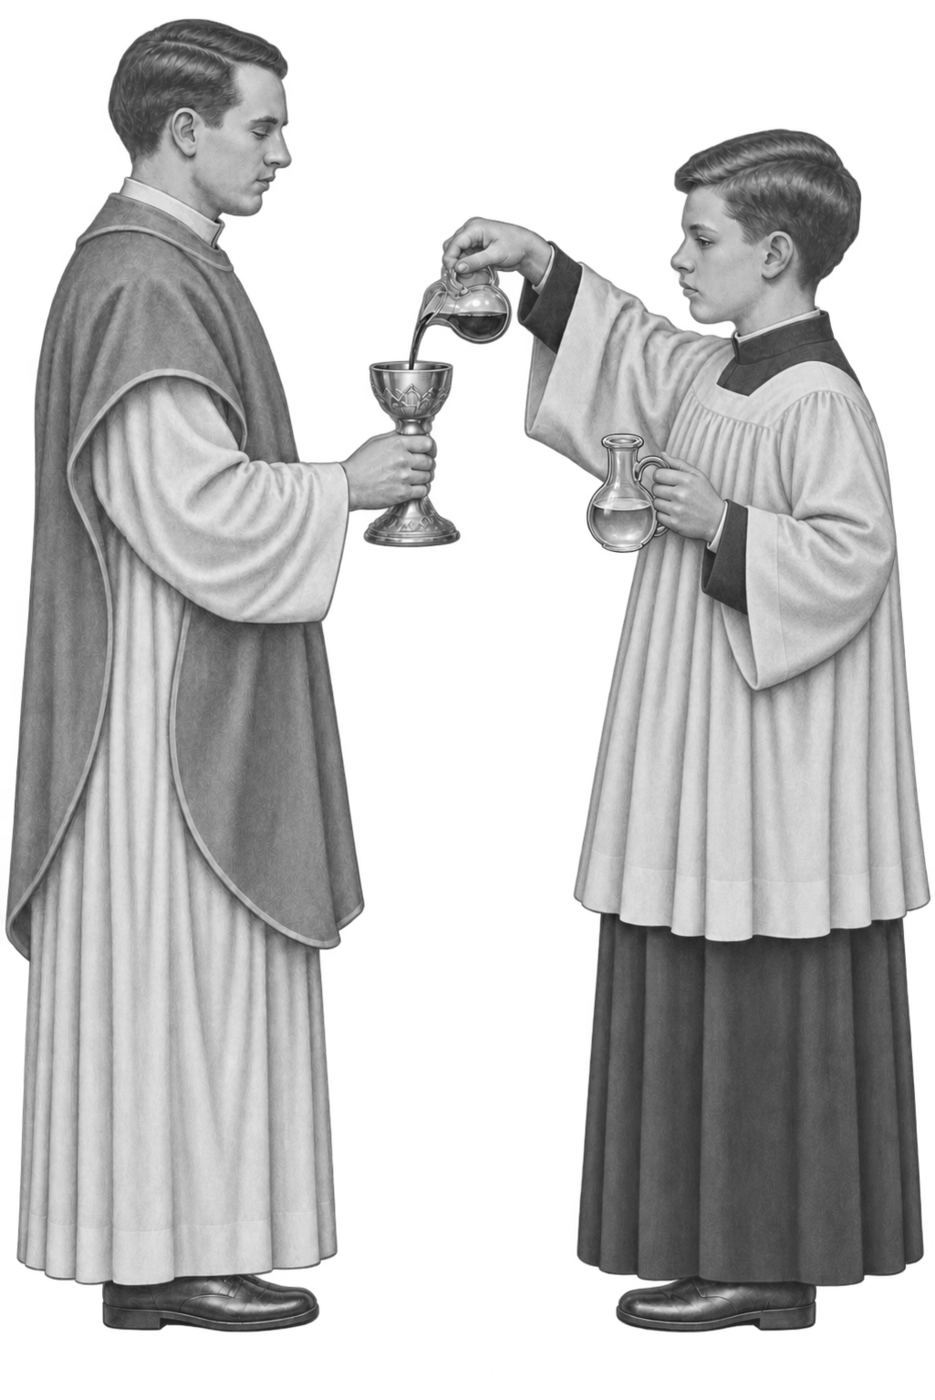
\includegraphics[#1]{liturgy/roman-rite/1962/reference/altar-server-guides/shared/artwork/pencil/ASG-ART-043-first-purification.png}}
\newcommand{\LMFingerWineArt}[1]{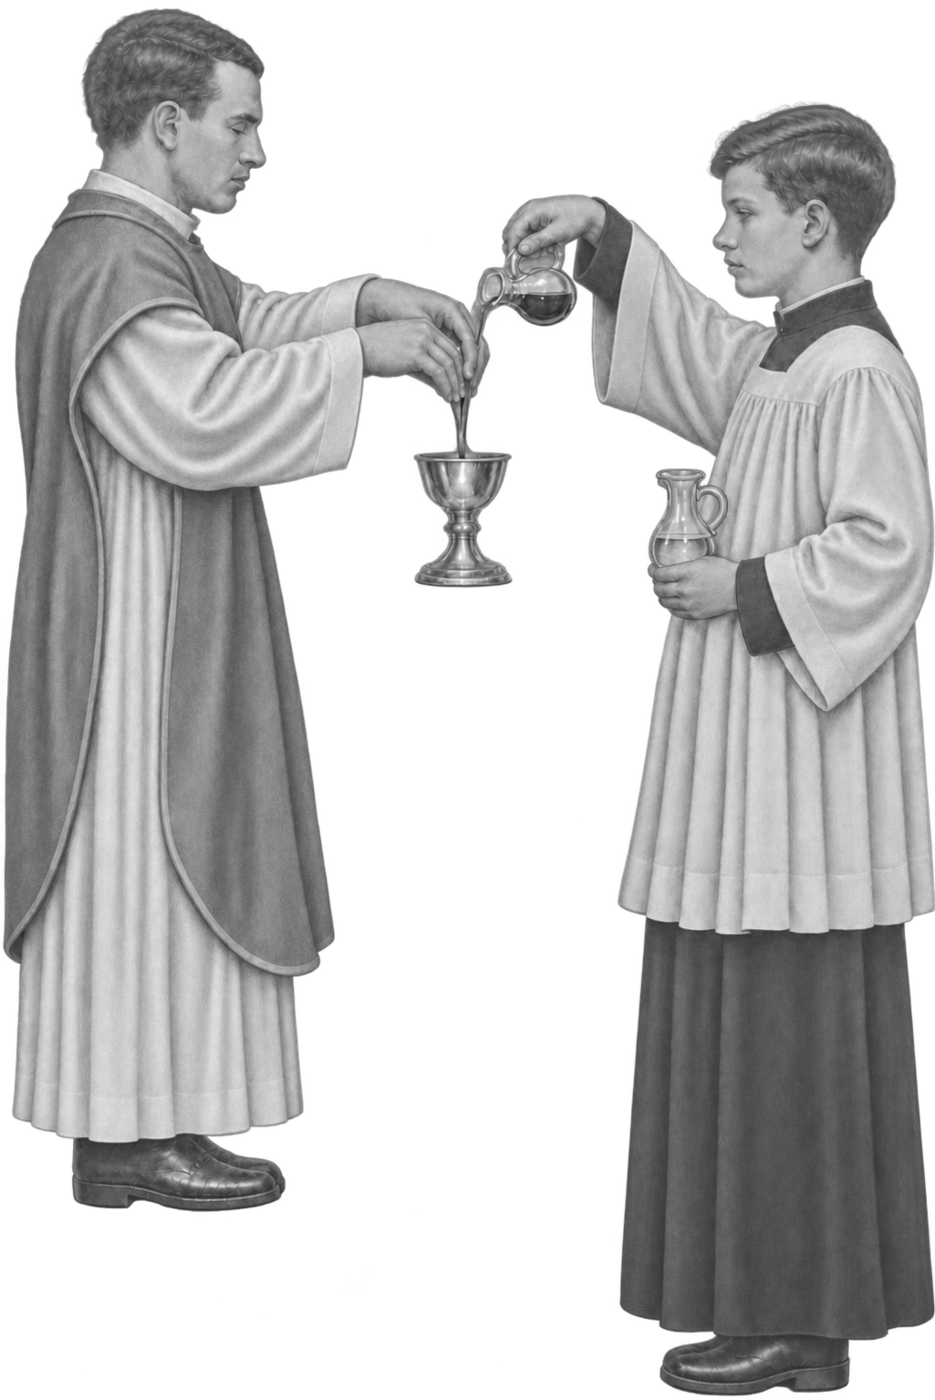
\includegraphics[#1]{liturgy/roman-rite/1962/reference/altar-server-guides/shared/artwork/pencil/ASG-ART-058-finger-ablution-wine-no-altar-v1.png}}
\newcommand{\LMFingerWaterArt}[1]{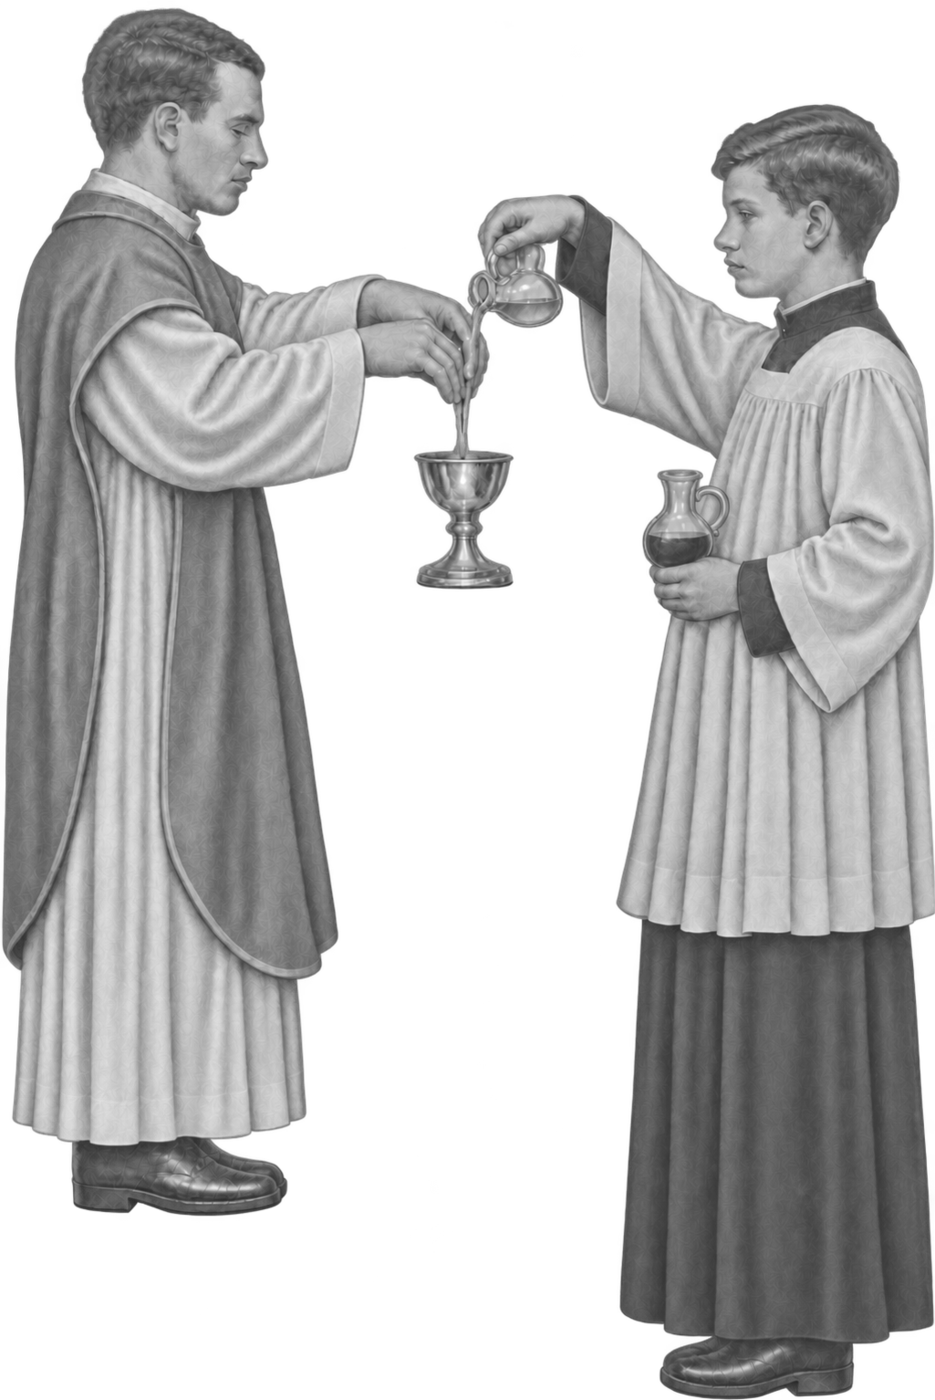
\includegraphics[#1]{liturgy/roman-rite/1962/reference/altar-server-guides/shared/artwork/pencil/ASG-ART-059-finger-ablution-water-no-altar-v1.png}}
\newcommand{\LMLavaboArt}[1]{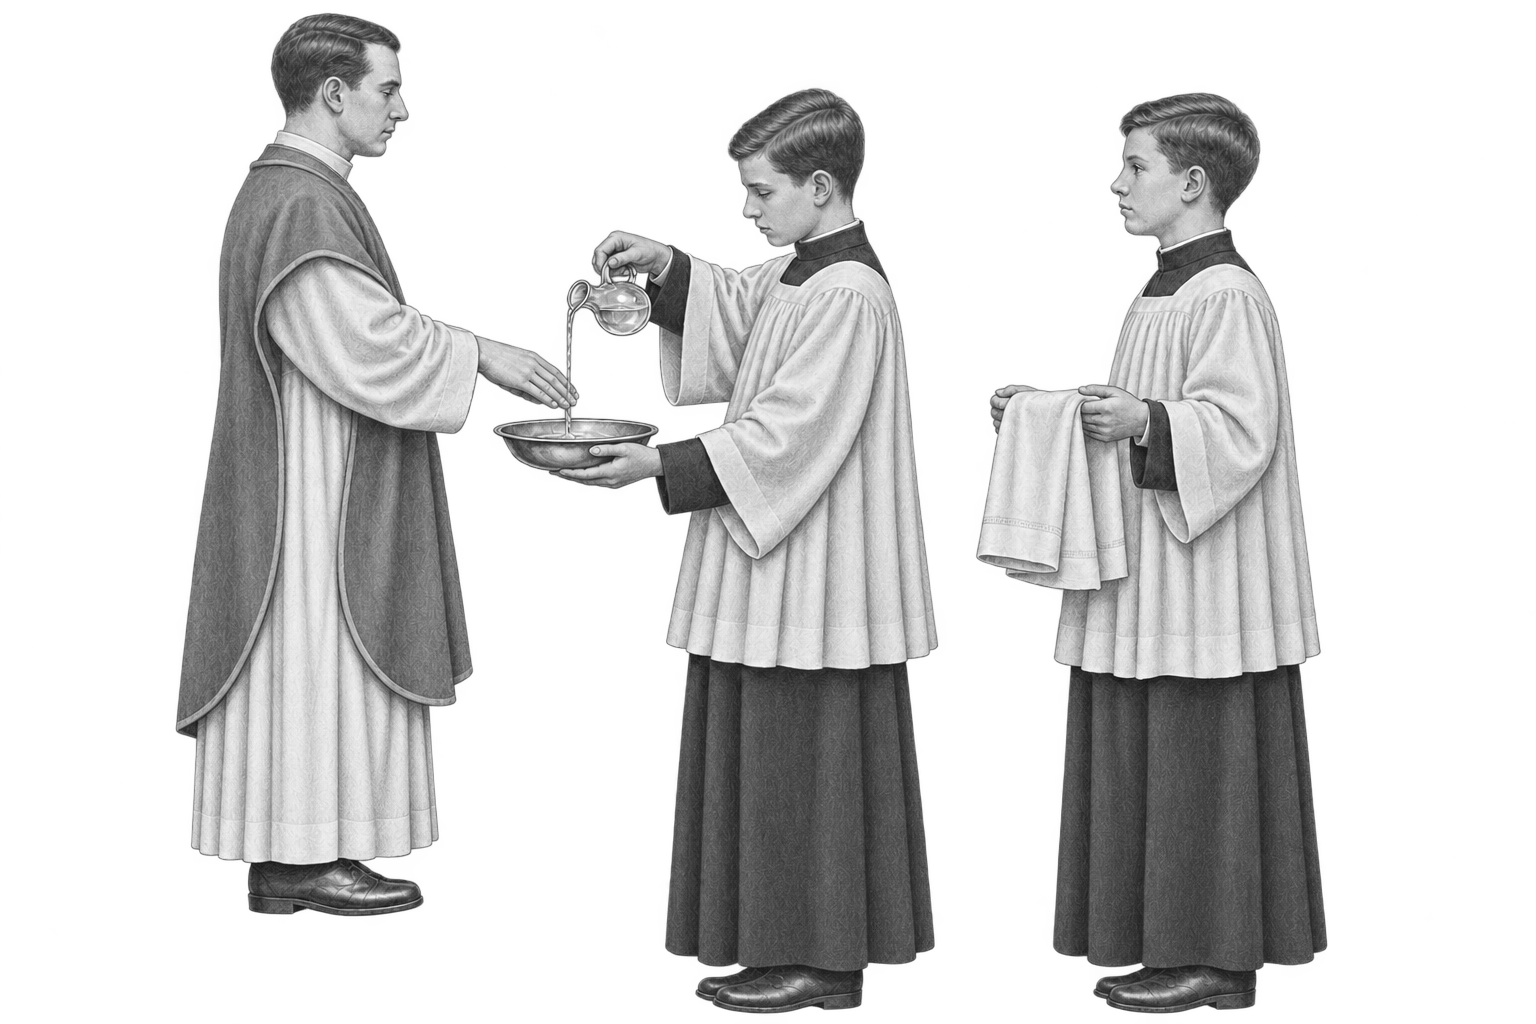
\includegraphics[#1]{liturgy/roman-rite/1962/reference/altar-server-guides/shared/artwork/pencil/ASG-ART-046-lavabo-service.png}}
\newcommand{\LMHostElevationArt}[1]{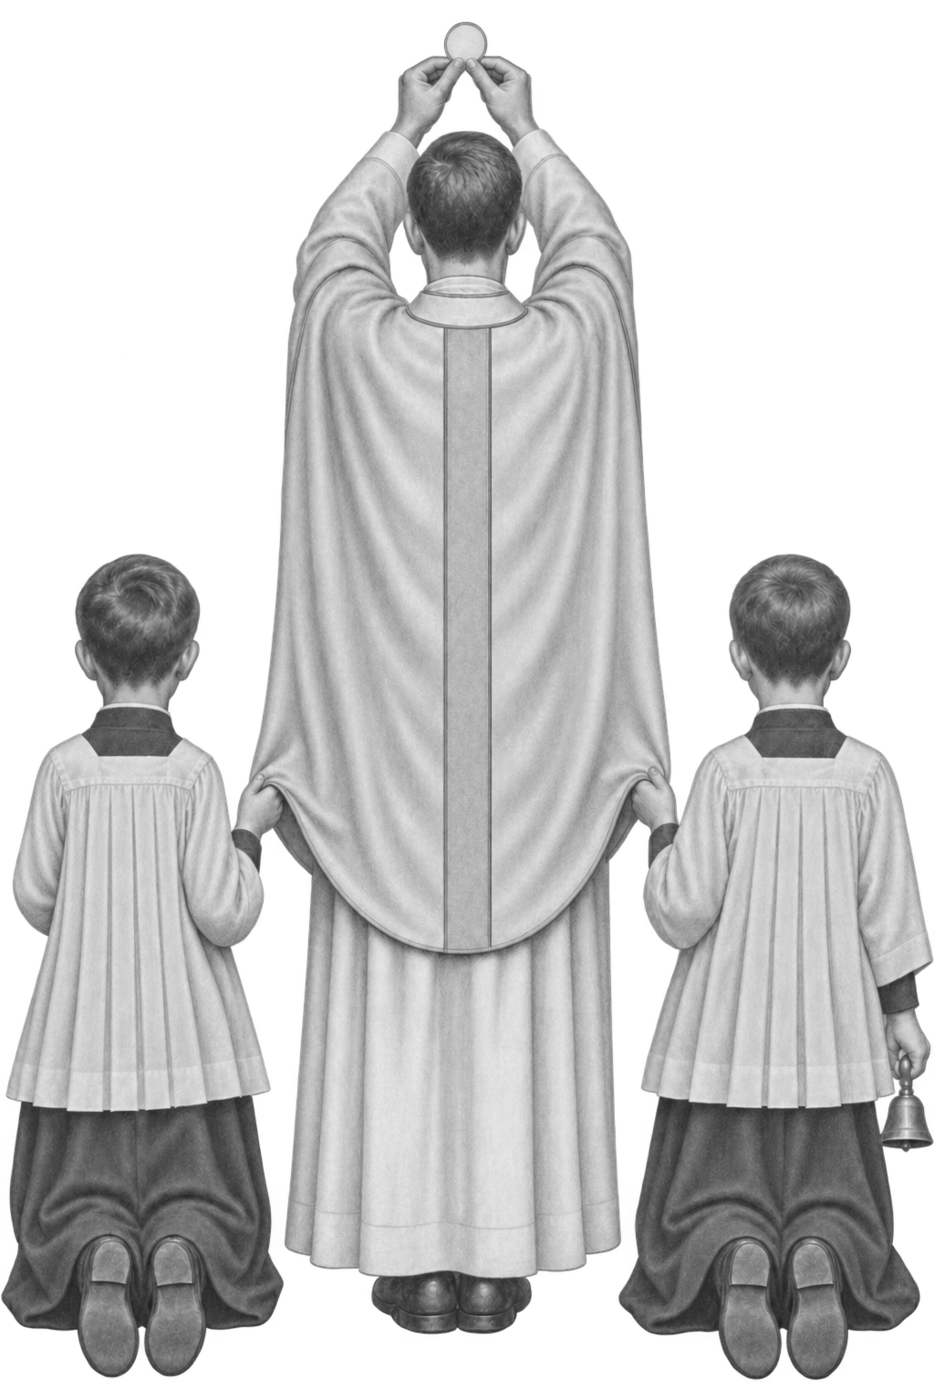
\includegraphics[#1]{liturgy/roman-rite/1962/reference/altar-server-guides/shared/artwork/pencil/ASG-ART-047-elevation-host.png}}
\newcommand{\LMChaliceElevationArt}[1]{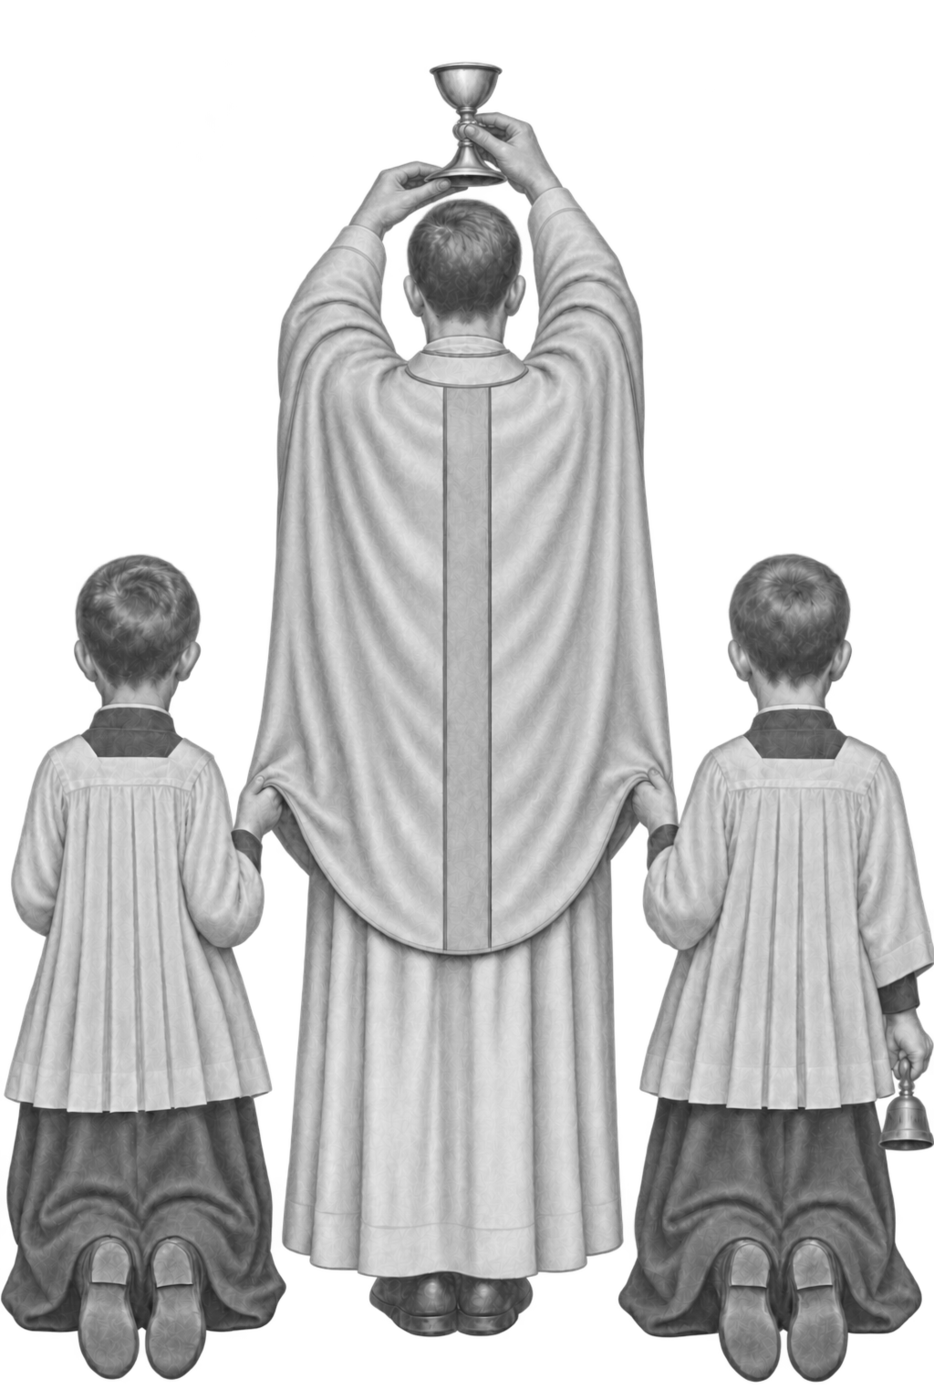
\includegraphics[#1]{liturgy/roman-rite/1962/reference/altar-server-guides/shared/artwork/pencil/ASG-ART-048-elevation-chalice.png}}
\newcommand{\LMChaliceBearer}[3]{%
  \node[anchor=south,inner sep=0pt] at (#1,#2) {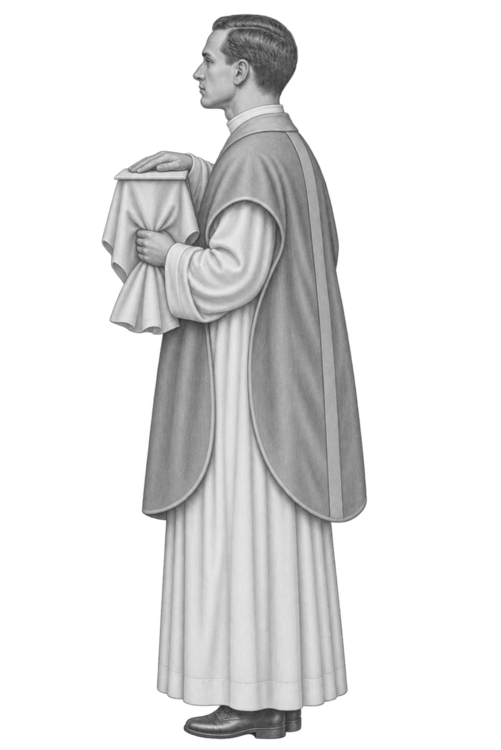
\includegraphics[height=28\ASGSceneUnit]{liturgy/roman-rite/1962/reference/altar-server-guides/shared/artwork/pencil/ASG-ART-051-priest-carrying-covered-chalice.png}};
  \ASGStation{#1}{#2-2}{#3}}
\newcommand{\LMVeilBearer}[3]{%
  \node[anchor=south,inner sep=0pt] at (#1,#2) {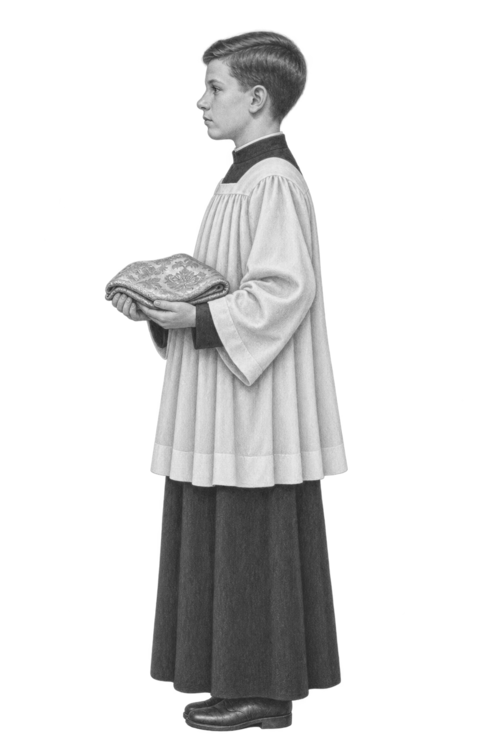
\includegraphics[height=23\ASGSceneUnit]{liturgy/roman-rite/1962/reference/altar-server-guides/shared/artwork/pencil/ASG-ART-052-server-carrying-folded-veil.png}};
  \ASGStation{#1}{#2-2}{#3}}

\newcommand{\LMSceneWinePresentation}{%
  \LMPositionScene{%
    \LMRestingLavaboTowel{93.6}{19.6}\LMRestingLavaboBasin{93.6}{19.2}
    \LMRestingCommunionPlate{91}{19.2}
    \LMMissalAtGospel\LMRestingVeil{70}{43}
    \node[anchor=south west,inner sep=0pt] at (61.3691,22.0)
      {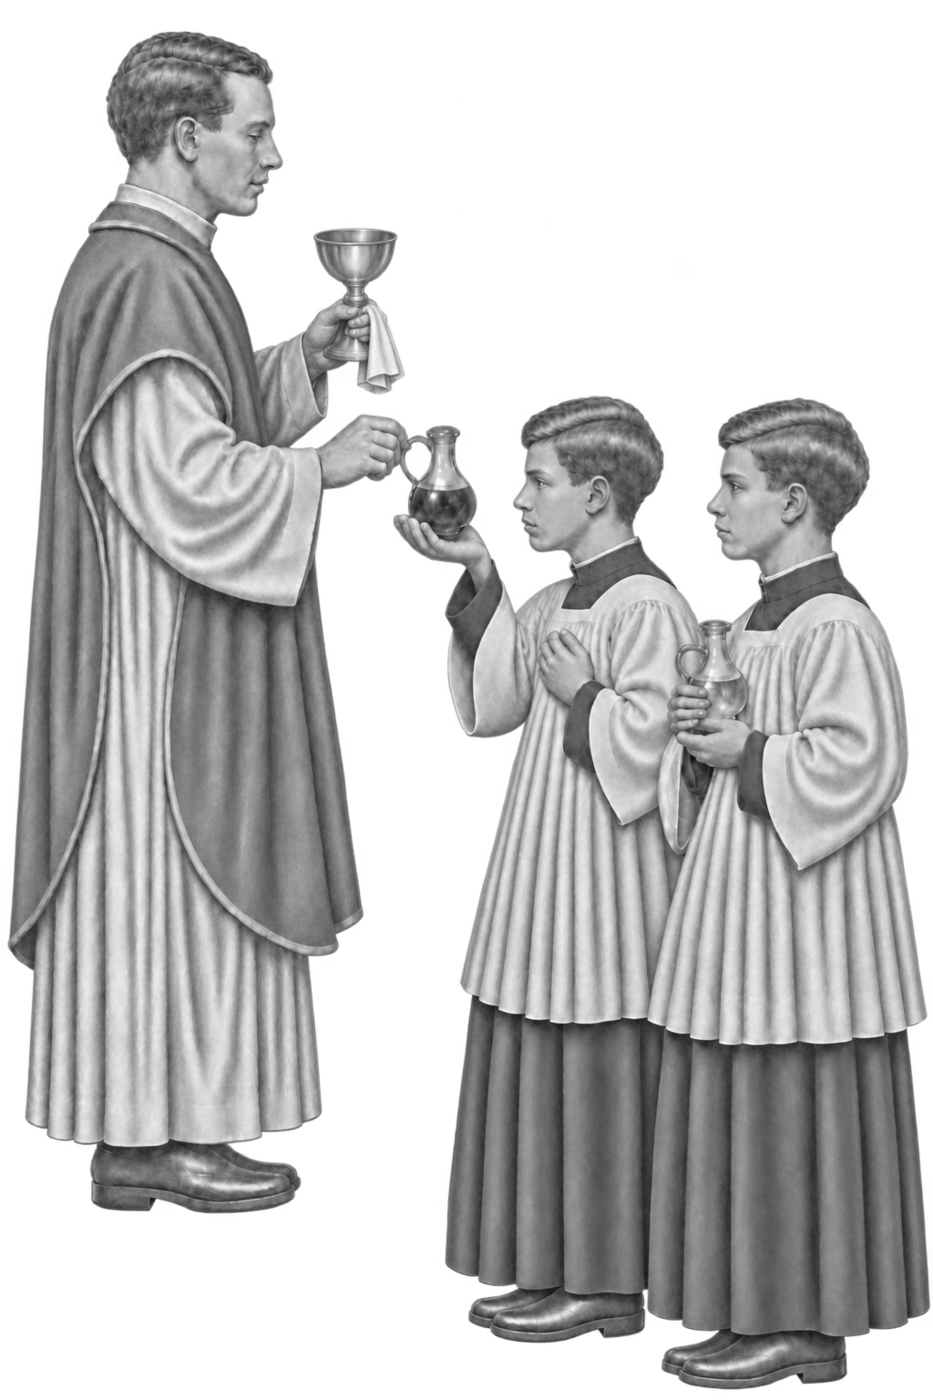
\includegraphics[height=33.4186\ASGSceneUnit]{liturgy/roman-rite/1962/reference/altar-server-guides/shared/artwork/pencil/ASG-ART-060-offertory-wine-handoff.png}};
    \ASGStation{66}{24}{PRIEST}\ASGStation{74}{20}{FIRST}\ASGStation{84}{16}{SECOND}
    \ASGStation{75}{5}{FIRST: WINE\quad SECOND: WATER}
  }{Wine handoff: First offers the handle; Second holds water and waits beside him on Step 2.}}
\newcommand{\LMSceneWaterPresentation}{%
  \LMPositionScene{%
    \LMRestingLavaboTowel{93.6}{19.6}\LMRestingLavaboBasin{93.6}{19.2}
    \LMRestingCommunionPlate{91}{19.2}
    \LMMissalAtGospel\LMRestingVeil{70}{43}
    \node[anchor=south west,inner sep=0pt] at (61.3691,22.0)
      {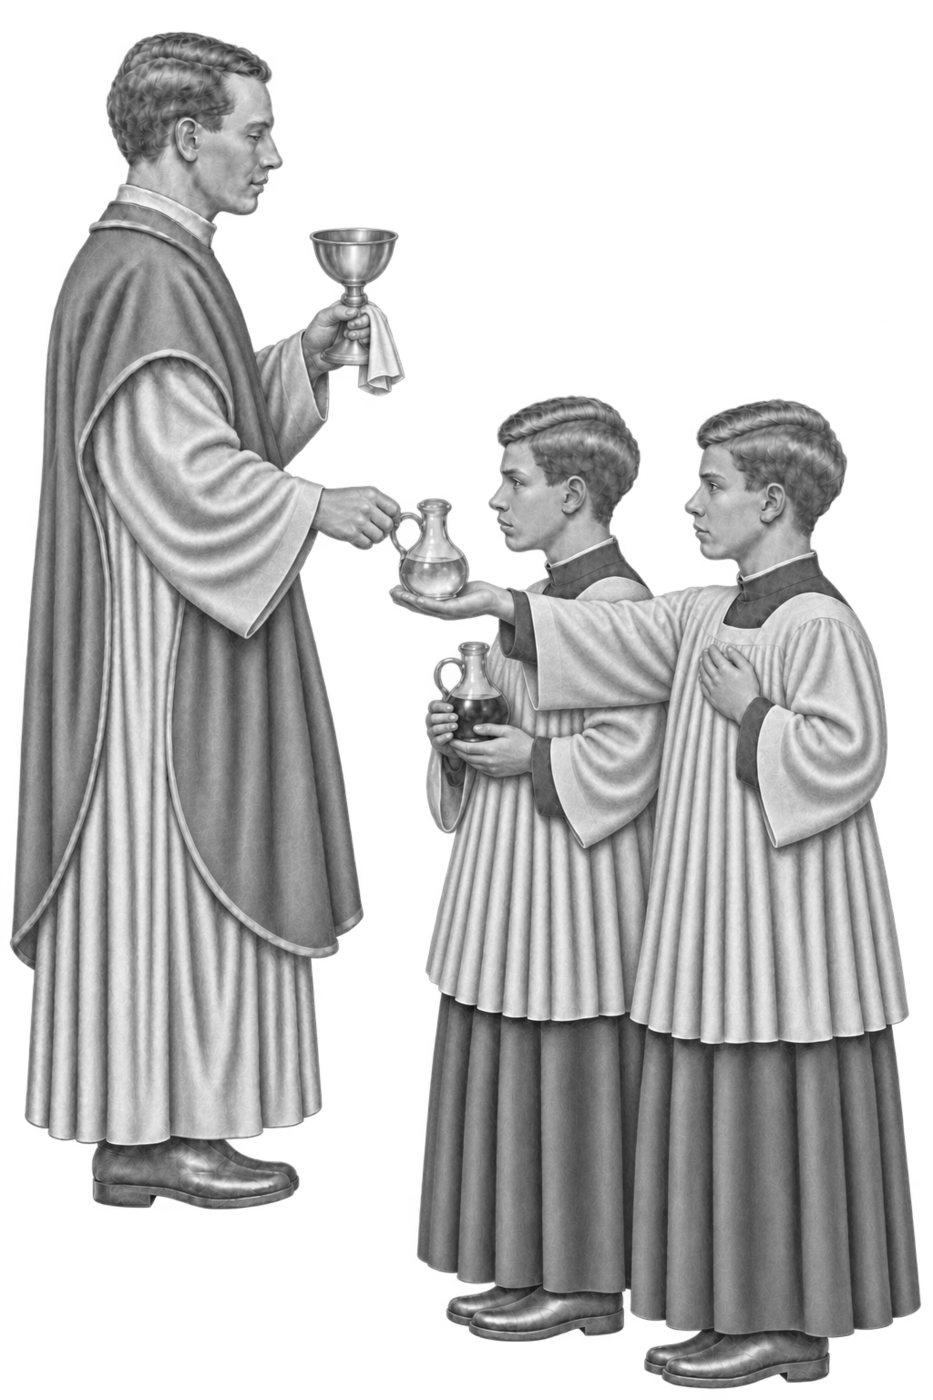
\includegraphics[height=33.4186\ASGSceneUnit]{liturgy/roman-rite/1962/reference/altar-server-guides/shared/artwork/pencil/ASG-ART-061-offertory-water-handoff.png}};
    \ASGStation{66}{24}{PRIEST}\ASGStation{74}{20}{FIRST}\ASGStation{84}{16}{SECOND}
    \ASGStation{75}{5}{SECOND: WATER\quad FIRST: WINE}
  }{Water handoff: Second offers the handle; First holds the returned wine. Neither changes place.}}
\newcommand{\LMCruetPresentationDetail}{%
  \LMSceneEnlargement{63}{34}{86}{53}{6.6cm}{The handle is free and faces the priest's receiving hand.}}
\newcommand{\LMCruetSequenceDetail}{%
  \noindent\begin{minipage}[t]{.49\linewidth}\vspace{0pt}\LMCruetKissDetail\end{minipage}\hfill
  \begin{minipage}[t]{.49\linewidth}\vspace{0pt}\LMCruetPresentationDetail\end{minipage}\par}

\newcommand{\LMSceneWinePurification}{%
  \LMPositionScene{%
    \LMRestingLavaboTowel{93.6}{19.6}\LMRestingLavaboBasin{93.6}{19.2}
    \LMRestingCommunionPlate{60}{43}
    \LMRestingBell{80}{22.5}
    \LMMissalAtGospel\LMRestingVeil{70}{43}\ASGStandingServer{25}{11.3}{SECOND\\WAITS}
    \node[anchor=south west,inner sep=0pt] at (46,26.5) {\LMWinePurificationArt{height=28\ASGSceneUnit,trim=0 67 0 19,clip}};
    \ASGStation{50}{24}{PRIEST}\ASGStation{64}{24}{FIRST}
    \ASGStation{73}{5}{FIRST WINE: BOTH ON PREDELLA}
  }{First wine purification: the priest holds the chalice; First pours into it.}}
\newcommand{\LMWinePurificationDetail}{%
  \LMSceneEnlargement{48}{38}{66}{52}{7.2cm}{Wine goes into the held chalice; the fingers are not being washed.}}

\newcommand{\LMSceneFingerWine}{%
  \LMPositionScene{%
    \LMRestingLavaboTowel{93.6}{19.6}\LMRestingLavaboBasin{93.6}{19.2}
    \LMRestingCommunionPlate{60}{43}
    \LMRestingBell{80}{22.5}
    \LMMissalAtGospel\LMRestingVeil{70}{43}\ASGStandingServer{25}{11.3}{SECOND\\WAITS}
    \node[anchor=south west,inner sep=0pt] at (53.5,22.5) {\LMFingerWineArt{height=35\ASGSceneUnit}};
    \ASGStation{59.5}{25}{PRIEST}\ASGStation{75.5}{20}{FIRST}
    \ASGStation{75}{5}{FINGERS: WINE FIRST}
  }{The priest stays on the predella; First pours from Step 2, at Epistle.}}
\newcommand{\LMFingerWineDetail}{%
  \LMSceneEnlargement{57.5}{38}{75.5}{52}{7.2cm}{Wine over both thumbs and forefingers; the chalice base rests on the altar.}}
\newcommand{\LMSceneFingerWater}{%
  \LMPositionScene{%
    \LMRestingLavaboTowel{93.6}{19.6}\LMRestingLavaboBasin{93.6}{19.2}
    \LMRestingCommunionPlate{60}{43}
    \LMRestingBell{80}{22.5}
    \LMMissalAtGospel\LMRestingVeil{70}{43}\ASGStandingServer{25}{11.3}{SECOND\\WAITS}
    \node[anchor=south west,inner sep=0pt] at (53.5,22.5) {\LMFingerWaterArt{height=35\ASGSceneUnit}};
    \ASGStation{59.5}{25}{PRIEST}\ASGStation{75.5}{20}{FIRST}
    \ASGStation{75}{5}{FINGERS: WATER NEXT}
  }{Same station, next pour: First follows with water; Second still waits clear.}}
\newcommand{\LMFingerWaterDetail}{%
  \LMSceneEnlargement{57.5}{38}{75.5}{52}{7.2cm}{Water over the same fingers into the same altar-supported chalice.}}

\newcommand{\LMSceneLavaboAction}{%
  \LMPositionScene{%
    \LMRestingCommunionPlate{91}{19.2}
    \LMChaliceWithPallObject{50}{43}
    \LMRestingWineCruet{97.2}{19.6}
    \LMMissalAtGospel\LMRestingVeil{70}{43}
    \node[anchor=south west,inner sep=0pt] at (50,23.2) {\LMLavaboArt{height=32\ASGSceneUnit,trim=160 10 200 10,clip}};
    \ASGStation{56}{25}{PRIEST}\ASGStation{70}{20}{SECOND}\ASGStation{82}{16}{FIRST}
    \ASGPairPlan{SECOND}{FIRST}
  }{Lavabo: Second pours into the bowl; First has the open towel ready.}}
\newcommand{\LMLavaboActionDetail}{%
  \LMSceneEnlargement{57}{35}{84}{49}{8.2cm}{Water and bowl belong to Second; the towel belongs to First.}}

\newcommand{\LMSceneHostElevation}{%
  \LMPositionScene{%
    \LMRestingLavaboTowel{93.6}{19.6}\LMRestingLavaboBasin{93.6}{19.2}
    \LMRestingCommunionPlate{91}{19.2}
    \LMChaliceWithPallObject{50}{43}
    \LMRestingCruets{97.2}{19.6}
    \LMMissalAtGospel\LMRestingVeil{70}{43}
    \node[anchor=south west,inner sep=0pt] at (38,25.5) {\LMHostElevationArt{height=34\ASGSceneUnit,trim=0 10 0 10,clip}};
    \ASGStation{50}{62}{PRIEST}
    \ASGStation{42}{23}{SECOND}\ASGStation{58}{23}{FIRST}
  }{Host elevation: both kneel, lift the nearest lower edge, and keep the priest's movement free.}}
\newcommand{\LMHostElevationDetail}{%
  \LMSceneEnlargement{39}{28}{62}{42}{7.6cm}{The inside hands lift the two edges; First's outside right hand rings the bell.}}
\newcommand{\LMSceneChaliceElevation}{%
  \LMPositionScene{%
    \LMRestingLavaboTowel{93.6}{19.6}\LMRestingLavaboBasin{93.6}{19.2}
    \LMRestingCommunionPlate{91}{19.2}
    \LMRestingCruets{97.2}{19.6}
    \LMMissalAtGospel\LMRestingVeil{70}{43}
    \node[anchor=south west,inner sep=0pt] at (38,25.5) {\LMChaliceElevationArt{height=34\ASGSceneUnit,trim=0 10 0 10,clip}};
    \ASGStation{50}{62}{PRIEST}
    \ASGStation{42}{23}{SECOND}\ASGStation{58}{23}{FIRST}
  }{Chalice elevation: the same two places and hand assignments; release when it is lowered.}}
\newcommand{\LMChaliceElevationDetail}{%
  \LMSceneEnlargement{39}{28}{62}{42}{7.6cm}{Repeat the lift and three rings, then release the chasuble and remain still.}}

% Successive movement states for the shared Low-Mass child/trainer course.
% Each frame has one figure per actor. Standing centre stops precede the
% reverence taught live; no picture purports to depict a genuflection.
% Only symmetric, two-handed carries and joined hands may be mirrored.
\newcommand{\LMMoveEmptyRight}[3]{%
  \node[anchor=south,inner sep=0pt] at (#1,#2) {\reflectbox{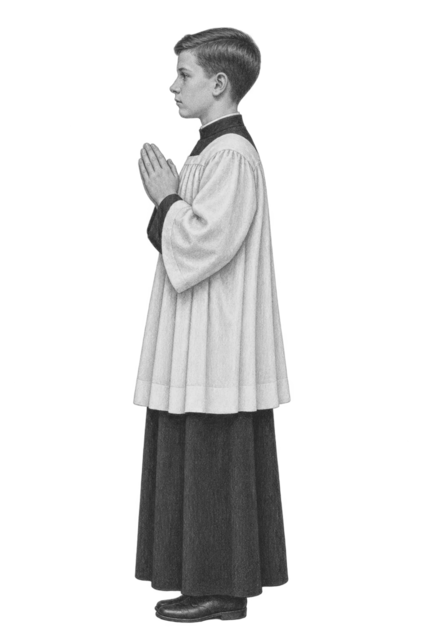
\includegraphics[height=23\ASGSceneUnit]{liturgy/roman-rite/1962/reference/altar-server-guides/shared/artwork/pencil/ASG-ART-037-server-facing-left.png}}};
  \ASGStation{#1}{#2-2}{#3}}
\newcommand{\LMMoveBookRight}[3]{%
  \node[anchor=south,inner sep=0pt] at (#1,#2) {\reflectbox{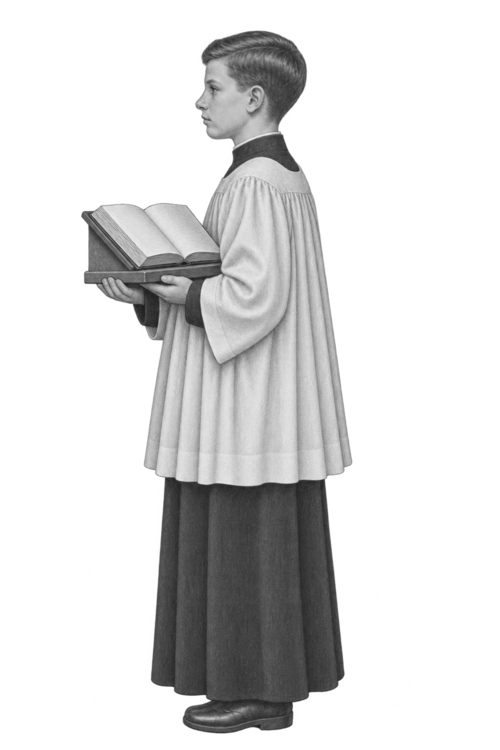
\includegraphics[height=23\ASGSceneUnit,trim=0 13 0 28,clip]{liturgy/roman-rite/1962/reference/altar-server-guides/shared/artwork/pencil/ASG-ART-040-server-carrying-missal.png}}};
  \ASGStation{#1}{#2-2}{#3}}
\newcommand{\LMMoveInstruction}[1]{%
  \par\smallskip{\fontsize{12}{14.5}\selectfont\RaggedRight #1\par}\smallskip}

\newcommand{\LMMoveBookRear}[3]{%
  \node[anchor=south,inner sep=0pt] at (#1,#2) {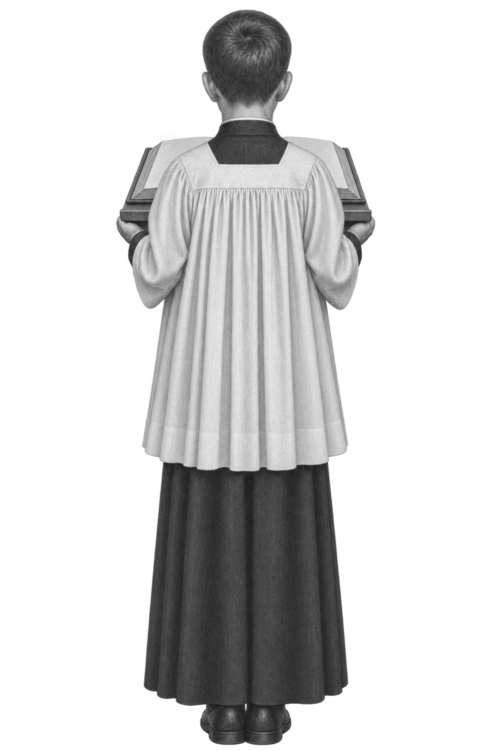
\includegraphics[height=23\ASGSceneUnit]{liturgy/roman-rite/1962/reference/altar-server-guides/shared/artwork/pencil/ASG-ART-053-server-carrying-missal-rear-v1.png}};
  \ASGStation{#1}{#2-2}{#3}}

\newcommand{\LMMoveMissalLift}{%
  \LMPositionScene{%
    \LMRestingCommunionPlate{91}{19.2}
    \LMRestingLavaboTowel{93.6}{19.6}\LMRestingLavaboBasin{93.6}{19.2}
    \LMCoveredChaliceObject{50}{43}
    \LMRestingCruets{97.2}{19.6}
    \ASGPriest{50}{26.5}{PRIEST}
    \ASGStandingServer{20}{11.3}{SECOND\\STAYS}
    \LMMoveBookRight{72}{26.5}{FIRST}
    \draw[asg route] (77,25) -- (81,23);
  }{1. First has lifted the Missal and stand together and turned toward the Epistle descent.}}
\newcommand{\LMMoveMissalDescent}{%
  \LMPositionScene{%
    \LMRestingCommunionPlate{91}{19.2}
    \LMRestingLavaboTowel{93.6}{19.6}\LMRestingLavaboBasin{93.6}{19.2}
    \LMCoveredChaliceObject{50}{43}
    \LMRestingCruets{97.2}{19.6}
    \ASGPriest{50}{26.5}{PRIEST}
    \ASGStandingServer{20}{11.3}{SECOND\\STAYS}
    \LMMoveBookRight{80}{18.3}{FIRST}
    \draw[asg route] (84,18) -- (86,12);
  }{2. First reaches the lowest step with both hands still supporting the book and stand.}}
\newcommand{\LMMoveMissalCentre}{%
  \LMPositionScene{%
    \LMRestingCommunionPlate{91}{19.2}
    \LMRestingLavaboTowel{93.6}{19.6}\LMRestingLavaboBasin{93.6}{19.2}
    \LMCoveredChaliceObject{50}{43}
    \LMRestingCruets{97.2}{19.6}
    \LMPriestAbove{50}{26.5}
    \ASGStandingServer{20}{11.3}{SECOND\\STAYS}
    \LMMoveBookRear{50}{11.3}{FIRST}
  }{3. At the centre, First stops and faces the altar with the book held securely.}}
\newcommand{\LMMoveMissalAscent}{%
  \LMPositionScene{%
    \LMRestingCommunionPlate{91}{19.2}
    \LMRestingLavaboTowel{93.6}{19.6}\LMRestingLavaboBasin{93.6}{19.2}
    \LMCoveredChaliceObject{50}{43}
    \LMRestingCruets{97.2}{19.6}
    \ASGPriest{50}{26.5}{PRIEST}
    \ASGStandingServer{20}{11.3}{SECOND\\STAYS}
    \LMMoveBookRear{31}{18.3}{FIRST}
    \draw[asg route] (36,19) -- (36,24);
  }{4. After the centre reverence, First turns up the Gospel steps with the book.}}
\newcommand{\LMMoveMissalPlaced}{%
  \LMPositionScene{%
    \LMRestingCommunionPlate{91}{19.2}
    \LMRestingLavaboTowel{93.6}{19.6}\LMRestingLavaboBasin{93.6}{19.2}
    \LMCoveredChaliceObject{50}{43}
    \LMRestingCruets{97.2}{19.6}
    \LMMissalAtGospel\ASGPriest{50}{26.5}{PRIEST}
    \ASGStandingServer{20}{11.3}{SECOND\\STAYS}
    \ASGStandingServer{31}{26.5}{FIRST}
  }{5. The book now rests at Gospel, angled toward the priest; First's hands are free.}}
\newcommand{\LMMoveMissalStepDown}{%
  \LMPositionScene{%
    \LMRestingCommunionPlate{91}{19.2}
    \LMRestingLavaboTowel{93.6}{19.6}\LMRestingLavaboBasin{93.6}{19.2}
    \LMCoveredChaliceObject{50}{43}
    \LMRestingCruets{97.2}{19.6}
    \LMMissalAtGospel\LMPriestFacingLeft{39}{26.5}{PRIEST}
    \ASGStandingServer{20}{11.3}{SECOND\\STAYS}
    \ASGStandingServer{29}{22.5}{FIRST}
  }{6. First has stepped down to Step 2 beside the book. Second has not moved up.}}
\newcommand{\LMMoveGospelDescent}{%
  \LMPositionScene{%
    \LMRestingCommunionPlate{91}{19.2}
    \LMRestingLavaboTowel{93.6}{19.6}\LMRestingLavaboBasin{93.6}{19.2}
    \LMCoveredChaliceObject{50}{43}
    \LMRestingCruets{97.2}{19.6}
    \LMMissalAtGospel\LMPriestFacingLeft{39}{26.5}{PRIEST}
    \ASGStandingServer{20}{11.3}{SECOND\\STAYS}
    \ASGServerFacingLeft{31}{18.3}{FIRST}
    \draw[asg route] (28,17) -- (28,12);
  }{1. Once the reading has begun, First steps down Gospel; the book stays on the altar.}}
\newcommand{\LMMoveGospelCentre}{%
  \LMPositionScene{%
    \LMRestingCommunionPlate{91}{19.2}
    \LMRestingLavaboTowel{93.6}{19.6}\LMRestingLavaboBasin{93.6}{19.2}
    \LMCoveredChaliceObject{50}{43}
    \LMRestingCruets{97.2}{19.6}
    \LMMissalAtGospel\LMPriestFacingLeft{39}{26.5}{PRIEST}
    \ASGStandingServer{20}{11.3}{SECOND\\STAYS}
    \ASGStandingServer{50}{11.3}{FIRST}
  }{2. First stops below the centre, faces the altar, and makes the taught reverence.}}
\newcommand{\LMMoveGospelCross}{%
  \LMPositionScene{%
    \LMRestingCommunionPlate{91}{19.2}
    \LMRestingLavaboTowel{93.6}{19.6}\LMRestingLavaboBasin{93.6}{19.2}
    \LMCoveredChaliceObject{50}{43}
    \LMRestingCruets{97.2}{19.6}
    \LMMissalAtGospel\LMPriestFacingLeft{39}{26.5}{PRIEST}
    \ASGStandingServer{20}{11.3}{SECOND\\STAYS}
    \LMMoveEmptyRight{62}{11.3}{FIRST}
    \draw[asg route] (66,7) -- (74,7);
  }{3. First walks along the floor toward Epistle, clear of the steps.}}
\newcommand{\LMMoveGospelReturned}{%
  \LMPositionScene{%
    \LMRestingCommunionPlate{91}{19.2}
    \LMRestingLavaboTowel{93.6}{19.6}\LMRestingLavaboBasin{93.6}{19.2}
    \LMCoveredChaliceObject{50}{43}
    \LMRestingCruets{97.2}{19.6}
    \LMMissalAtGospel\LMPriestFacingLeft{39}{26.5}{PRIEST}
    \ASGStandingServer{20}{11.3}{SECOND\\STAYS}
    \ASGServerFacingLeft{75}{11.3}{FIRST}
  }{4. At the normal Epistle place, First turns toward the Gospel. Both remain below the steps.}}

% Offertory: the named veil point is this guide's rehearsed Epistle pickup
% point, not a claim that every sanctuary uses this spot.
\newcommand{\LMMoveVeilSetDown}{%
  \LMPositionScene{%
    \LMUncoveredChaliceObject{60}{43}
    \LMRestingCommunionPlate{91}{19.2}
    \LMRestingLavaboTowel{93.6}{19.6}\LMRestingLavaboBasin{93.6}{19.2}
    \LMRestingCruets{97.2}{19.6}
    \LMMissalAtGospel\ASGPriest{50}{26.5}{PRIEST}
    \LMRestingVeil{70}{43}
    \ASGStandingServer{73}{26.5}{FIRST}
    \ASGStandingServer{25}{11.3}{SECOND\\WAITS}
    \ASGStation{82}{58}{VEIL PICKUP\\POINT}
  }{1. First has set the folded veil at the marked Epistle point; his hands are free.}}
\newcommand{\LMMoveVeilDescent}{%
  \LMPositionScene{%
    \LMUncoveredChaliceObject{60}{43}
    \LMRestingCommunionPlate{91}{19.2}
    \LMRestingLavaboTowel{93.6}{19.6}\LMRestingLavaboBasin{93.6}{19.2}
    \LMRestingCruets{97.2}{19.6}
    \LMMissalAtGospel\ASGPriest{50}{26.5}{PRIEST}
    \LMRestingVeil{70}{43}
    \LMMoveEmptyRight{80}{18.3}{FIRST}
    \ASGStandingServer{25}{11.3}{SECOND\\WAITS}
    \draw[asg route] (84,17) -- (84,12);
  }{2. First descends empty-handed. The folded veil stays at the same Epistle point.}}
\newcommand{\LMMoveOffertoryCentre}{%
  \LMPositionScene{%
    \LMUncoveredChaliceObject{60}{43}
    \LMRestingCommunionPlate{91}{19.2}
    \LMRestingLavaboTowel{93.6}{19.6}\LMRestingLavaboBasin{93.6}{19.2}
    \LMRestingCruets{97.2}{19.6}
    \LMMissalAtGospel\LMPriestAbove{50}{26.5}
    \LMRestingVeil{70}{43}
    \ASGStandingServer{57}{11.3}{FIRST}
    \ASGStandingServer{43}{11.3}{SECOND}
  }{3. Both meet on the floor at the centre, facing the altar with empty hands.}}
\newcommand{\LMMoveCredenceArrival}{%
  \LMPositionScene{%
    \LMUncoveredChaliceObject{60}{43}
    \LMRestingCommunionPlate{91}{19.2}
    \LMRestingLavaboTowel{93.6}{19.6}\LMRestingLavaboBasin{93.6}{19.2}
    \LMMissalAtGospel\ASGPriest{50}{26.5}{PRIEST}
    \LMRestingVeil{70}{43}\LMRestingCruets{97.2}{19.6}
    \LMMoveEmptyRight{83}{11.3}{FIRST}
    \LMMoveEmptyRight{70}{11.3}{SECOND}
    \draw[asg route] (76,6) -- (86,6);
  }{4. After the centre reverence, both reach the credence. The cruets are still on it.}}
\newcommand{\LMMoveCruetsTaken}{%
  \LMPositionScene{%
    \LMUncoveredChaliceObject{60}{43}
    \LMRestingCommunionPlate{91}{19.2}
    \LMRestingLavaboTowel{93.6}{19.6}\LMRestingLavaboBasin{93.6}{19.2}
    \LMMissalAtGospel\ASGPriest{50}{26.5}{PRIEST}
    \LMRestingVeil{70}{43}
    \LMWaitingCruetServer{75}{11.3}{FIRST}{2}
    \LMWaitingCruetServer{86}{11.3}{SECOND}{5}
    \ASGStation{74}{3}{FIRST: WINE\quad SECOND: WATER}
  }{5. First has taken wine and Second water. Both open cruets stay upright.}}
\newcommand{\LMMoveCruetsAscent}{%
  \LMPositionScene{%
    \LMUncoveredChaliceObject{60}{43}
    \LMRestingCommunionPlate{91}{19.2}
    \LMRestingLavaboTowel{93.6}{19.6}\LMRestingLavaboBasin{93.6}{19.2}
    \LMMissalAtGospel\ASGPriestFacingRight{66}{26.5}{PRIEST}
    \LMRestingVeil{70}{43}
    \LMWaitingCruetServer{75}{18.3}{FIRST}{2}
    \LMWaitingCruetServer{84}{18.3}{SECOND}{5}
    \draw[asg route] (70,19) -- (70,22);
  }{6. At the first step, both still hold their own cruets; continue to the Step 2 service place.}}
\newcommand{\LMMoveCruetsReset}{%
  \LMPositionScene{%
    \LMChaliceWithPallObject{50}{43}
    \LMRestingCommunionPlate{91}{19.2}
    \LMRestingLavaboTowel{93.6}{19.6}\LMRestingLavaboBasin{93.6}{19.2}
    \LMMissalAtGospel\ASGPriest{50}{26.5}{PRIEST}
    \LMRestingVeil{70}{43}\LMRestingCruets{97.2}{19.6}
    \LMMoveEmptyRight{83}{11.3}{FIRST}
    \LMMoveEmptyRight{71}{11.3}{SECOND}
  }{1. Back at the credence, both cruets are set down before the Lavabo equipment is taken.}}
\newcommand{\LMMoveLavaboEquipped}{%
  \LMPositionScene{%
    \LMChaliceWithPallObject{50}{43}
    \LMRestingCommunionPlate{91}{19.2}
    \LMRestingWineCruet{97.2}{19.6}
    \LMMissalAtGospel\ASGPriest{50}{26.5}{PRIEST}
    \LMRestingVeil{70}{43}
    \LMMoveTowelRear{85}{11.3}{FIRST}
    \LMMoveBowlRear{73}{11.3}{SECOND}
  }{2. First now holds the open towel; Second holds the bowl and upright water cruet.}}
\newcommand{\LMMoveLavaboAscent}{%
  \LMPositionScene{%
    \LMChaliceWithPallObject{50}{43}
    \LMRestingCommunionPlate{91}{19.2}
    \LMRestingWineCruet{97.2}{19.6}
    \LMMissalAtGospel\ASGPriestFacingRight{61}{26.5}{PRIEST}
    \LMRestingVeil{70}{43}
    \LMMoveTowelRear{81}{18.3}{FIRST}
    \LMMoveBowlRear{70}{18.3}{SECOND}
    \draw[asg route] (67,19) -- (67,22);
  }{3. Carry the changed equipment up Epistle: Second keeps bowl and water level, First keeps the towel clear.}}
\newcommand{\LMMoveBellTaken}{%
  \LMPositionScene{%
    \LMChaliceWithPallObject{50}{43}
    \LMRestingCommunionPlate{91}{19.2}
    \LMRestingLavaboTowel{93.6}{19.6}\LMRestingLavaboBasin{93.6}{19.2}
    \LMMissalAtGospel\ASGPriest{50}{26.5}{PRIEST}
    \LMRestingVeil{70}{43}\LMRestingCruets{97.2}{19.6}
    \LMMoveBellRear{80}{11.3}{FIRST}
    \ASGStandingServer{68}{11.3}{SECOND}
  }{1. Lavabo articles are reset. First now holds the bell; Second's hands are free.}}
\newcommand{\LMMoveBellCentre}{%
  \LMPositionScene{%
    \LMChaliceWithPallObject{50}{43}
    \LMRestingCommunionPlate{91}{19.2}
    \LMRestingLavaboTowel{93.6}{19.6}\LMRestingLavaboBasin{93.6}{19.2}
    \LMRestingCruets{97.2}{19.6}
    \LMMissalAtGospel\LMPriestAbove{50}{26.5}
    \LMRestingVeil{70}{43}
    \LMMoveBellAtAltar{57}{11.3}{FIRST}
    \ASGStandingServer{43}{11.3}{SECOND}
  }{2. Both stop facing the altar at the centre. First keeps the bell still during the reverence.}}
\newcommand{\LMMoveBellAtNormalPlace}{%
  \LMPositionScene{%
    \LMChaliceWithPallObject{50}{43}
    \LMRestingCommunionPlate{91}{19.2}
    \LMRestingLavaboTowel{93.6}{19.6}\LMRestingLavaboBasin{93.6}{19.2}
    \LMRestingCruets{97.2}{19.6}
    \LMMissalAtGospel\ASGPriest{50}{26.5}{PRIEST}
    \LMRestingVeil{70}{43}
    \LMMoveBellAtAltar{75}{11.3}{FIRST}
    \ASGStandingServer{25}{11.3}{SECOND}
  }{3. Both have returned to their normal floor places. First still holds the bell before setting it down.}}

\newcommand{\LMMoveCruetsRear}[3]{%
  \node[anchor=south,inner sep=0pt] at (#1,#2) {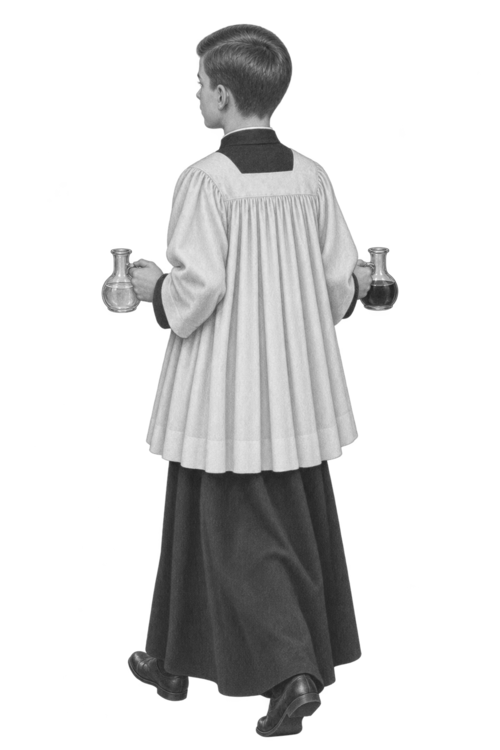
\includegraphics[height=23\ASGSceneUnit]{liturgy/roman-rite/1962/reference/altar-server-guides/shared/artwork/pencil/ASG-ART-054-server-carrying-two-cruets-v1.png}};
  \ASGStation{#1}{#2-2}{#3}}

\newcommand{\LMMoveBellRear}[3]{%
  \node[anchor=south,inner sep=0pt] at (#1,#2) {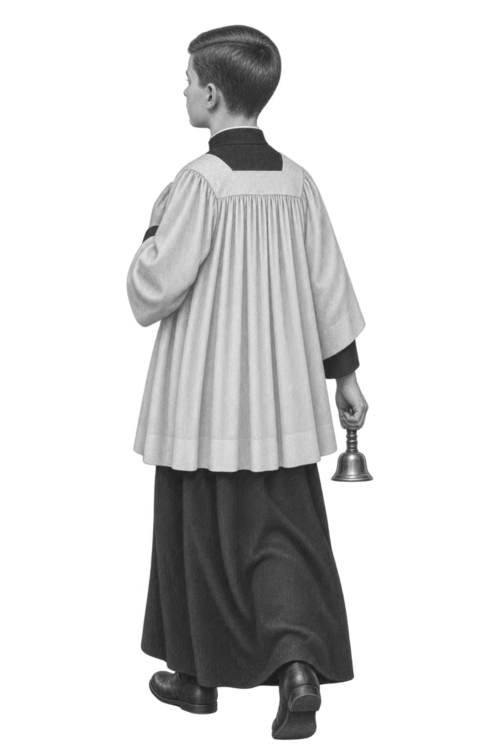
\includegraphics[height=23\ASGSceneUnit]{liturgy/roman-rite/1962/reference/altar-server-guides/shared/artwork/pencil/ASG-ART-055-server-carrying-bell-right-v1.png}};
  \ASGStation{#1}{#2-2}{#3}}

\newcommand{\LMMoveBowlRear}[3]{%
  \node[anchor=south,inner sep=0pt] at (#1,#2) {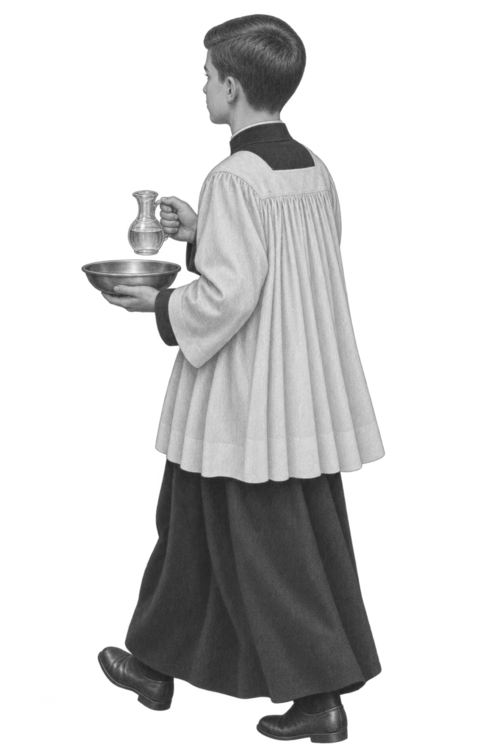
\includegraphics[height=23\ASGSceneUnit]{liturgy/roman-rite/1962/reference/altar-server-guides/shared/artwork/pencil/ASG-ART-056-server-carrying-bowl-water-v1.png}};
  \ASGStation{#1}{#2-2}{#3}}

\newcommand{\LMMoveTowelRear}[3]{%
  \node[anchor=south,inner sep=0pt] at (#1,#2) {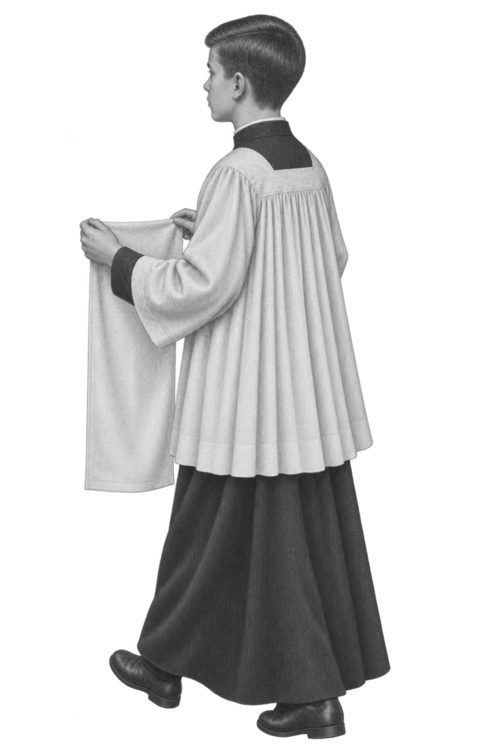
\includegraphics[height=23\ASGSceneUnit]{liturgy/roman-rite/1962/reference/altar-server-guides/shared/artwork/pencil/ASG-ART-057-server-carrying-open-towel-v1.png}};
  \ASGStation{#1}{#2-2}{#3}}

\newcommand{\LMMoveLavaboReady}{%
  \LMPositionScene{%
    \LMChaliceWithPallObject{50}{43}
    \LMRestingCommunionPlate{91}{19.2}
    \LMRestingWineCruet{97.2}{19.6}
    \LMMissalAtGospel\ASGPriestFacingRight{61}{26.5}{PRIEST}
    \LMRestingVeil{70}{43}
    \LMMoveTowelRear{81}{22.5}{FIRST}
    \LMMoveBowlRear{70}{22.5}{SECOND}
  }{4. Both arrive at Step 2 with the same equipment. Stop, bow together, and face the priest before washing.}}

\newcommand{\LMMoveElevationFirstStep}{%
  \LMPositionScene{%
    \LMChaliceWithPallObject{50}{43}
    \LMRestingCommunionPlate{91}{19.2}
    \LMRestingLavaboTowel{93.6}{19.6}\LMRestingLavaboBasin{93.6}{19.2}
    \LMRestingCruets{97.2}{19.6}
    \LMMissalAtGospel\ASGPriest{50}{26.5}{PRIEST}
    \LMRestingVeil{70}{43}
    \LMMoveBellRear{74}{18.3}{FIRST}
    \ASGStandingServer{26}{18.3}{SECOND}
    \draw[asg route] (69,19) -- (64,22);
    \draw[asg route] (31,19) -- (36,22);
  }{1. After the warning, both have risen and begun the short ascent. First carries the bell in his right hand.}}

\newcommand{\LMMoveElevationSecondStep}{%
  \LMPositionScene{%
    \LMChaliceWithPallObject{50}{43}
    \LMRestingCommunionPlate{91}{19.2}
    \LMRestingLavaboTowel{93.6}{19.6}\LMRestingLavaboBasin{93.6}{19.2}
    \LMRestingCruets{97.2}{19.6}
    \LMMissalAtGospel\ASGPriest{50}{26.5}{PRIEST}
    \LMRestingVeil{70}{43}
    \LMMoveBellRear{62}{22.5}{FIRST}
    \ASGStandingServer{38}{22.5}{SECOND}
  }{2. Both reach Step 2 on their own sides; next ascend to the predella and kneel slightly behind the priest.}}

\newcommand{\LMMoveElevationDescent}{%
  \LMPositionScene{%
    \LMChaliceWithPallObject{50}{43}
    \LMRestingCommunionPlate{91}{19.2}
    \LMRestingLavaboTowel{93.6}{19.6}\LMRestingLavaboBasin{93.6}{19.2}
    \LMRestingCruets{97.2}{19.6}
    \LMMissalAtGospel\ASGPriest{50}{26.5}{PRIEST}
    \LMRestingVeil{70}{43}
    \LMMoveBellFront{64}{18.3}{FIRST}
    \LMMoveEmptyRight{36}{18.3}{SECOND}
    \draw[asg route] (63,17) -- (60,12);
    \draw[asg route] (35,17) -- (40,12);
  }{1. After the final reverence, both descend. First keeps the bell upright and silent.}}

\newcommand{\LMMoveElevationCentre}{%
  \LMPositionScene{%
    \LMChaliceWithPallObject{50}{43}
    \LMRestingCommunionPlate{91}{19.2}
    \LMRestingLavaboTowel{93.6}{19.6}\LMRestingLavaboBasin{93.6}{19.2}
    \LMRestingCruets{97.2}{19.6}
    \LMMissalAtGospel\LMPriestAbove{50}{26.5}
    \LMRestingVeil{70}{43}
    \LMMoveBellAtAltar{57}{11.3}{FIRST}
    \ASGStandingServer{43}{11.3}{SECOND}
  }{2. Both stop on the floor facing the altar. First still has the bell for the centre reverence.}}

\newcommand{\LMMoveAblutionTaken}{%
  \LMPositionScene{%
    \LMRestingCommunionPlate{60}{43}
    \LMUncoveredChaliceObject{50}{43}
    \LMRestingLavaboTowel{93.6}{19.6}\LMRestingLavaboBasin{93.6}{19.2}
    \LMRestingBell{80}{22.5}
    \LMMissalAtGospel\ASGPriest{50}{26.5}{PRIEST}
    \LMRestingVeil{70}{43}
    \ASGStandingServer{25}{11.3}{SECOND\\WAITS}
    \LMMoveCruetsRear{83}{11.3}{FIRST}
  }{1. First leaves the credence with wine in his right hand and water in his left. Second is standing below Gospel.}}

\newcommand{\LMMoveAblutionAscent}{%
  \LMPositionScene{%
    \LMRestingCommunionPlate{60}{43}
    \LMUncoveredChaliceObject{50}{43}
    \LMRestingLavaboTowel{93.6}{19.6}\LMRestingLavaboBasin{93.6}{19.2}
    \LMRestingBell{80}{22.5}
    \LMMissalAtGospel\ASGPriest{50}{26.5}{PRIEST}
    \LMRestingVeil{70}{43}
    \ASGStandingServer{25}{11.3}{SECOND\\WAITS}
    \LMMoveCruetsRear{78}{18.3}{FIRST}
    \draw[asg route] (73,19) -- (73,22);
  }{2. First carries both upright cruets up Epistle toward Step 2; Second leaves the lane clear.}}

\newcommand{\LMMoveAblutionStepTwo}{%
  \LMPositionScene{%
    \LMRestingCommunionPlate{60}{43}
    \LMUncoveredChaliceObject{50}{43}
    \LMRestingLavaboTowel{93.6}{19.6}\LMRestingLavaboBasin{93.6}{19.2}
    \LMRestingBell{80}{22.5}
    \LMMissalAtGospel\ASGPriest{50}{26.5}{PRIEST}
    \LMRestingVeil{70}{43}
    \ASGStandingServer{25}{11.3}{SECOND\\WAITS}
    \LMMoveCruetsRear{76}{22.5}{FIRST}
  }{3. First reaches the waiting step at Epistle. Stop here until the priest offers the chalice.}}

\newcommand{\LMMoveAblutionPredella}{%
  \LMPositionScene{%
    \LMRestingCommunionPlate{60}{43}
    \LMRestingLavaboTowel{93.6}{19.6}\LMRestingLavaboBasin{93.6}{19.2}
    \LMRestingBell{80}{22.5}
    \LMMissalAtGospel\LMMovePriestWithChalice{50}{26.5}{PRIEST}
    \LMRestingVeil{70}{43}
    \ASGStandingServer{25}{11.3}{SECOND\\WAITS}
    \LMMoveCruetsRear{68}{26.5}{FIRST}
    \draw[asg route] (63,25) -- (59,25);
  }{4. At the priest's cue, First has ascended to the predella and approaches the centre with both cruets.}}

\newcommand{\LMMoveAblutionDown}{%
  \LMPositionScene{%
    \LMRestingCommunionPlate{60}{43}
    \LMRestingLavaboTowel{93.6}{19.6}\LMRestingLavaboBasin{93.6}{19.2}
    \LMRestingBell{80}{22.5}
    \LMMissalAtGospel\LMMovePriestWithChalice{50}{26.5}{PRIEST}
    \LMRestingVeil{70}{43}
    \ASGStandingServer{25}{11.3}{SECOND\\WAITS}
    \LMMoveCruetsFront{76}{22.5}{FIRST}
  }{After the first wine pour, First steps back down to Step 2 carrying both cruets; wait for the priest to come to Epistle.}}

\newcommand{\LMMoveAblutionReturn}{%
  \LMPositionScene{%
    \LMRestingCommunionPlate{60}{43}
    \LMUncoveredChaliceObject{44}{43}
    \LMRestingLavaboTowel{93.6}{19.6}\LMRestingLavaboBasin{93.6}{19.2}
    \LMRestingBell{80}{22.5}
    \LMMissalAtGospel\ASGPriest{63}{26.5}{PRIEST}
    \LMRestingVeil{70}{43}
    \ASGStandingServer{25}{11.3}{SECOND\\WAITS}
    \LMMoveCruetsFront{81}{18.3}{FIRST}
    \draw[asg route] (85,17) -- (88,12);
  }{1. After the water pour and the priest's signal, First descends with both cruets to return them to the credence.}}

\newcommand{\LMMoveAblutionReset}{%
  \LMPositionScene{%
    \LMRestingCommunionPlate{60}{43}
    \LMUncoveredChaliceObject{44}{43}
    \LMRestingLavaboTowel{93.6}{19.6}\LMRestingLavaboBasin{93.6}{19.2}
    \LMRestingBell{80}{22.5}
    \LMMissalAtGospel\ASGPriest{50}{26.5}{PRIEST}
    \LMRestingVeil{70}{43}
    \ASGStandingServer{25}{11.3}{SECOND\\WAITS}
    \LMRestingCruets{97.2}{19.6}
    \LMMoveEmptyRight{83}{11.3}{FIRST}
  }{2. Both cruets are back on the credence. First is empty-handed before any cleared Communion plate is retrieved.}}

\newcommand{\LMMoveExchangeTaken}{%
  \LMPositionScene{%
    \LMUncoveredChaliceObject{44}{43}
    \LMRestingCommunionPlate{91}{19.2}
    \LMRestingLavaboTowel{93.6}{19.6}\LMRestingLavaboBasin{93.6}{19.2}
    \LMRestingCruets{97.2}{19.6}\LMRestingBell{80}{22.5}
    \ASGPriest{50}{26.5}{PRIEST}
    \LMBookBearer{29}{18.3}{SECOND}
    \LMMoveVeilRight{78}{18.3}{FIRST}
  }{1. Second descends Gospel with the Missal and stand; First descends Epistle with the folded veil.}}

\newcommand{\LMMoveExchangeYield}{%
  \LMPositionScene{%
    \LMUncoveredChaliceObject{44}{43}
    \LMRestingCommunionPlate{91}{19.2}
    \LMRestingLavaboTowel{93.6}{19.6}\LMRestingLavaboBasin{93.6}{19.2}
    \LMRestingCruets{97.2}{19.6}\LMRestingBell{80}{22.5}
    \LMPriestAbove{50}{26.5}
    \LMMoveBookRight{55}{11.3}{SECOND}
    \LMVeilBearer{76}{11.3}{FIRST}
    \ASGStop{68}{8}{A}
    \draw[asg route] (60,8) -- (66,8);
    \ASGStation{79}{51}{FIRST WAITS\\BEFORE A}
  }{2. At the marked floor crossing A, First waits with the veil while Second passes toward Epistle with the book.}}

\newcommand{\LMMoveExchangeClear}{%
  \LMPositionScene{%
    \LMUncoveredChaliceObject{44}{43}
    \LMRestingCommunionPlate{91}{19.2}
    \LMRestingLavaboTowel{93.6}{19.6}\LMRestingLavaboBasin{93.6}{19.2}
    \LMRestingCruets{97.2}{19.6}\LMRestingBell{80}{22.5}
    \LMPriestAbove{50}{26.5}
    \LMMoveBookRear{76}{18.3}{SECOND}
    \LMVeilBearer{58}{11.3}{FIRST}
    \ASGStop{68}{8}{A}
    \draw[asg route] (52,7) -- (44,7);
  }{3. Second has cleared A and is going up Epistle. First can now cross below the steps toward Gospel.}}

\newcommand{\LMMoveExchangeBookPlaced}{%
  \LMPositionScene{%
    \LMUncoveredChaliceObject{44}{43}
    \LMRestingCommunionPlate{91}{19.2}
    \LMRestingLavaboTowel{93.6}{19.6}\LMRestingLavaboBasin{93.6}{19.2}
    \LMRestingCruets{97.2}{19.6}\LMRestingBell{80}{22.5}
    \ASGPriest{50}{26.5}{PRIEST}
    \LMMissalAtEpistle
    \ASGStandingServer{73}{26.5}{SECOND}
    \LMVeilBearer{29}{18.3}{FIRST}
    \draw[asg route] (25,19) -- (25,24);
  }{4. The Missal and stand now rest straight at Epistle. First reaches the Gospel steps with the veil.}}

\newcommand{\LMMoveExchangeVeilPlaced}{%
  \LMPositionScene{%
    \LMUncoveredChaliceObject{44}{43}
    \LMRestingCommunionPlate{91}{19.2}
    \LMRestingLavaboTowel{93.6}{19.6}\LMRestingLavaboBasin{93.6}{19.2}
    \LMRestingCruets{97.2}{19.6}\LMRestingBell{80}{22.5}
    \ASGPriest{50}{26.5}{PRIEST}
    \LMMissalAtEpistle\LMRestingVeil{31}{43}
    \ASGStandingServer{29}{26.5}{FIRST}
    \ASGStandingServer{73}{26.5}{SECOND}
  }{5. The folded veil now rests at the Gospel point. Both have released their objects and have empty hands.}}

\newcommand{\LMMoveExchangeEmptyDescent}{%
  \LMPositionScene{%
    \LMUncoveredChaliceObject{44}{43}
    \LMRestingCommunionPlate{91}{19.2}
    \LMRestingLavaboTowel{93.6}{19.6}\LMRestingLavaboBasin{93.6}{19.2}
    \LMRestingCruets{97.2}{19.6}\LMRestingBell{80}{22.5}
    \ASGPriest{50}{26.5}{PRIEST}
    \LMMissalAtEpistle\LMRestingVeil{31}{43}
    \ASGServerFacingLeft{28}{18.3}{FIRST}
    \LMMoveEmptyRight{78}{18.3}{SECOND}
    \draw[asg route] (25,17) -- (25,12);
    \draw[asg route] (82,17) -- (82,12);
  }{6. Both descend empty-handed from the sides where they placed the objects.}}

\newcommand{\LMMoveExchangeCentre}{%
  \LMPositionScene{%
    \LMUncoveredChaliceObject{44}{43}
    \LMRestingCommunionPlate{91}{19.2}
    \LMRestingLavaboTowel{93.6}{19.6}\LMRestingLavaboBasin{93.6}{19.2}
    \LMRestingCruets{97.2}{19.6}\LMRestingBell{80}{22.5}
    \LMPriestAbove{50}{26.5}
    \LMMissalAtEpistle\LMRestingVeil{31}{43}
    \ASGStandingServer{43}{11.3}{FIRST}
    \ASGStandingServer{57}{11.3}{SECOND}
  }{7. Both stop facing the altar at the centre. Make the taught reverence before returning to the normal sides.}}

\newcommand{\LMMoveExchangeReturn}{%
  \LMPositionScene{%
    \LMUncoveredChaliceObject{44}{43}
    \LMRestingCommunionPlate{91}{19.2}
    \LMRestingLavaboTowel{93.6}{19.6}\LMRestingLavaboBasin{93.6}{19.2}
    \LMRestingCruets{97.2}{19.6}\LMRestingBell{80}{22.5}
    \ASGPriest{50}{26.5}{PRIEST}
    \LMMissalAtEpistle\LMRestingVeil{31}{43}
    \LMMoveEmptyRight{66}{11.3}{FIRST}
    \ASGServerFacingLeft{33}{11.3}{SECOND}
    \draw[asg route] (68,6) -- (75,6);
    \draw[asg route] (31,6) -- (25,6);
  }{8. Following the rehearsed passing order, First returns toward Epistle and Second toward Gospel, both empty-handed.}}

\newcommand{\LMMoveEndingServers}{%
  \LMPositionScene{%
    \LMRestingCommunionPlate{91}{19.2}
    \LMRestingLavaboTowel{93.6}{19.6}\LMRestingLavaboBasin{93.6}{19.2}
    \LMRestingCruets{97.2}{19.6}\LMRestingBell{80}{22.5}
    \LMMissalAtEpistle\LMCoveredChaliceObject{50}{43}\ASGPriest{50}{26.5}{PRIEST}
    \LMMoveEmptyRight{29}{11.3}{SECOND}
    \ASGServerFacingLeft{71}{11.3}{FIRST}
    \draw[asg route] (32,6) -- (40,6);
    \draw[asg route] (68,6) -- (60,6);
  }{1. After the Last Gospel, both move inward along the floor toward the foot; the priest remains at the altar.}}

\newcommand{\LMMoveEndingPriestDown}{%
  \LMPositionScene{%
    \LMRestingCommunionPlate{91}{19.2}
    \LMRestingLavaboTowel{93.6}{19.6}\LMRestingLavaboBasin{93.6}{19.2}
    \LMRestingCruets{97.2}{19.6}\LMRestingBell{80}{22.5}
    \LMMissalAtEpistle
    \LMMovePriestChaliceFront{50}{18.3}{PRIEST}
    \ASGStandingServer{33}{11.3}{SECOND}
    \ASGStandingServer{67}{11.3}{FIRST}
  }{2. The priest descends carrying the covered chalice. The servers wait at the foot with the centre clear.}}

\newcommand{\LMMoveEndingForm}{%
  \LMPositionScene{%
    \LMRestingCommunionPlate{91}{19.2}
    \LMRestingLavaboTowel{93.6}{19.6}\LMRestingLavaboBasin{93.6}{19.2}
    \LMRestingCruets{97.2}{19.6}\LMRestingBell{80}{22.5}
    \LMMissalAtEpistle
    \LMChaliceBearer{50}{11.3}{PRIEST}
    \ASGServerFacingLeft{20}{11.3}{FIRST}
    \ASGServerFacingLeft{35}{11.3}{SECOND}
  }{After the common floor reverence, both turn into the departure line: First leads, Second follows, then the priest.}}

\newcommand{\LMMoveBellFront}[3]{%
  \node[anchor=south,inner sep=0pt] at (#1,#2) {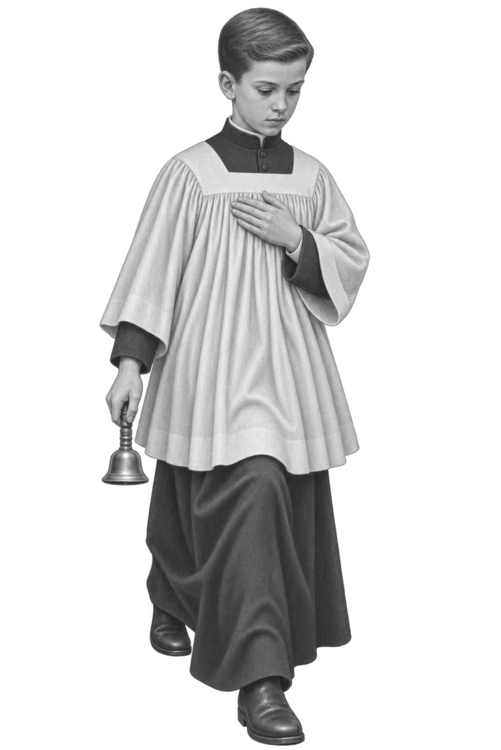
\includegraphics[height=23\ASGSceneUnit]{liturgy/roman-rite/1962/reference/altar-server-guides/shared/artwork/pencil/ASG-ART-064-server-descending-bell-right-v1.png}};
  \ASGStation{#1}{#2-2}{#3}}

\newcommand{\LMMoveCruetsFront}[3]{%
  \node[anchor=south,inner sep=0pt] at (#1,#2) {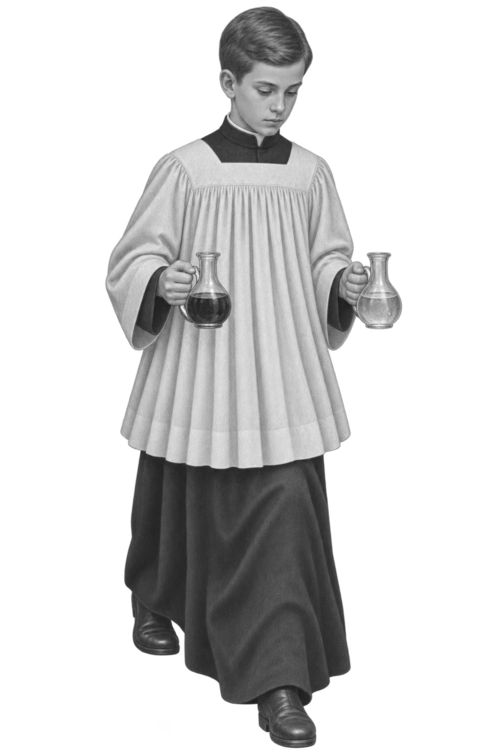
\includegraphics[height=23\ASGSceneUnit]{liturgy/roman-rite/1962/reference/altar-server-guides/shared/artwork/pencil/ASG-ART-065-server-descending-two-cruets-v1.png}};
  \ASGStation{#1}{#2-2}{#3}}

\newcommand{\LMMovePriestChaliceFront}[3]{%
  \node[anchor=south,inner sep=0pt] at (#1,#2) {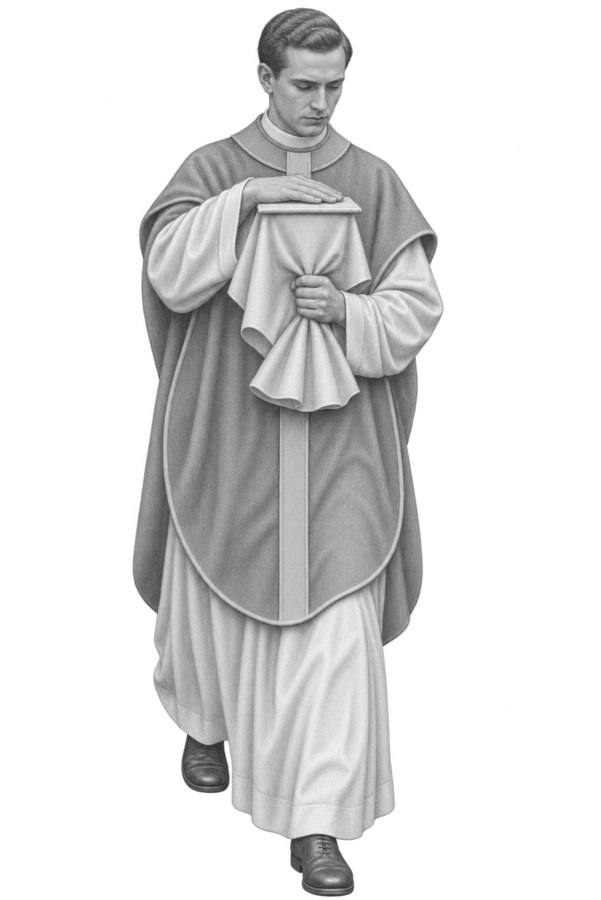
\includegraphics[height=28\ASGSceneUnit]{liturgy/roman-rite/1962/reference/altar-server-guides/shared/artwork/pencil/ASG-ART-066-priest-descending-covered-chalice-v1.png}};
  \ASGStation{#1}{#2-2}{#3}}

\newcommand{\LMMoveBellAtAltar}[3]{%
  \node[anchor=south,inner sep=0pt] at (#1,#2) {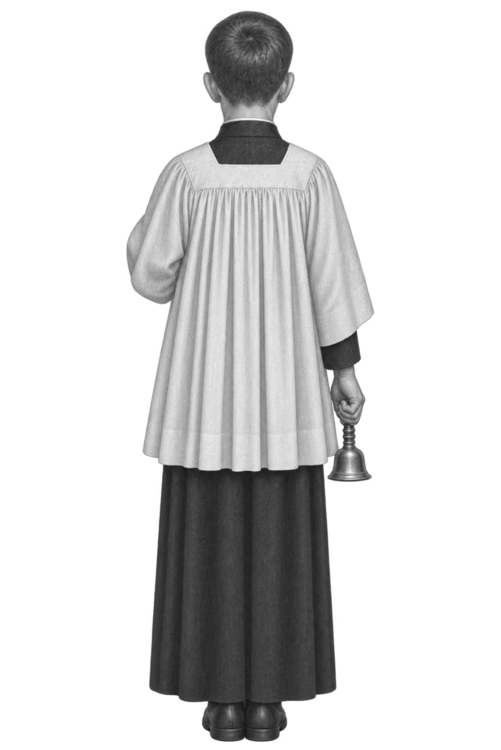
\includegraphics[height=23\ASGSceneUnit]{liturgy/roman-rite/1962/reference/altar-server-guides/shared/artwork/pencil/ASG-ART-067-server-standing-bell-right-rear-v1.png}};
  \ASGStation{#1}{#2-2}{#3}}

\newcommand{\LMMovePriestWithChalice}[3]{%
  \node[anchor=south,inner sep=0pt] at (#1,#2) {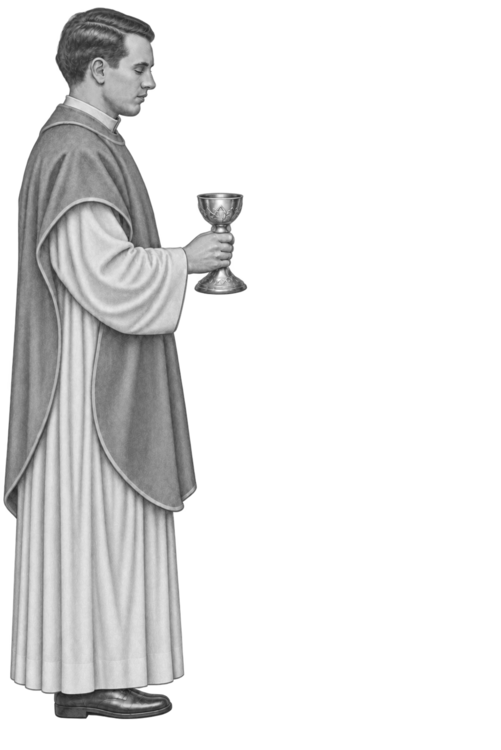
\includegraphics[height=28\ASGSceneUnit,trim=0 30 245 7,clip]{liturgy/roman-rite/1962/reference/altar-server-guides/shared/artwork/pencil/ASG-ART-075-priest-holding-uncovered-chalice.png}};
  \ASGStation{#1}{#2-2}{#3}}


% The rear priest is an orientation silhouette at this stopped moment. The
% covered chalice remains held in front and is honestly occluded by his body.
\newcommand{\LMMoveArrivalLine}{%
  \LMPositionScene{%
    \LMRestingCommunionPlate{91}{19.2}
    \LMRestingLavaboTowel{93.6}{19.6}\LMRestingLavaboBasin{93.6}{19.2}
    \LMRestingCruets{97.2}{19.6}
    \LMMissalAtEpistle
    \ASGServerFacingLeft{41}{11.3}{FIRST}
    \ASGServerFacingLeft{59}{11.3}{SECOND}
    \LMChaliceBearer{79}{11.3}{PRIEST}
    \draw[asg route] (35,6) -- (28,6);
  }{First leads, Second follows, and the priest carries the covered chalice behind them.}}
\newcommand{\LMMoveArrivalFacing}{%
  \LMPositionScene{%
    \LMRestingCommunionPlate{91}{19.2}
    \LMRestingLavaboTowel{93.6}{19.6}\LMRestingLavaboBasin{93.6}{19.2}
    \LMRestingCruets{97.2}{19.6}
    \LMMissalAtEpistle
    \ASGPriest{50}{11.3}{PRIEST}
    \ASGStandingServer{67}{11.3}{FIRST}
    \ASGStandingServer{33}{11.3}{SECOND}
  }{All have stopped facing the altar. The priest still holds the covered chalice in front, hidden by his back.}}
\newcommand{\LMMoveDepartureFacing}{%
  \LMPositionScene{%
    \LMRestingCommunionPlate{91}{19.2}
    \LMRestingLavaboTowel{93.6}{19.6}\LMRestingLavaboBasin{93.6}{19.2}
    \LMRestingCruets{97.2}{19.6}\LMRestingBell{80}{22.5}
    \LMMissalAtEpistle
    \ASGPriest{50}{11.3}{PRIEST}
    \ASGStandingServer{67}{11.3}{FIRST}
    \ASGStandingServer{33}{11.3}{SECOND}
  }{3. At the foot, all stop facing the altar. The priest's covered chalice remains held in front, hidden by his back.}}

\newcommand{\LMMoveVeilRight}[3]{%
  \node[anchor=south,inner sep=0pt] at (#1,#2) {\reflectbox{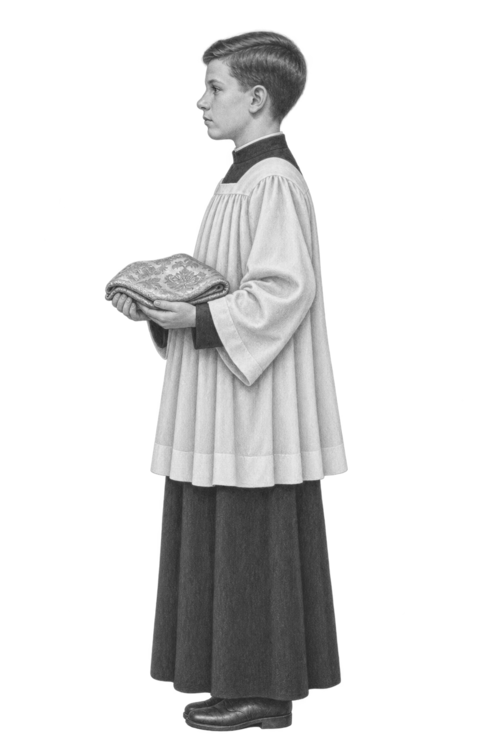
\includegraphics[height=23\ASGSceneUnit]{liturgy/roman-rite/1962/reference/altar-server-guides/shared/artwork/pencil/ASG-ART-052-server-carrying-folded-veil.png}}};
  \ASGStation{#1}{#2-2}{#3}}


% The plate carry is symmetric: both hands support the handle and underside.
% Its return view may be mirrored; no handed liturgical action is reversed.
\newcommand{\LMMovePlateLeft}[3]{%
  \node[anchor=south,inner sep=0pt] at (#1,#2) {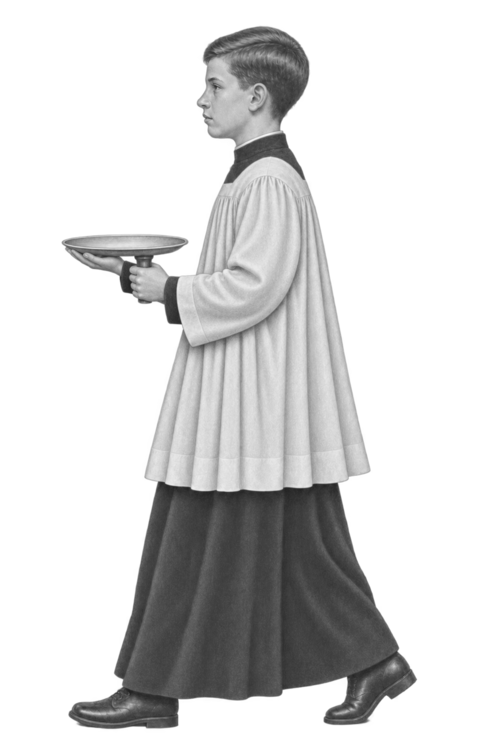
\includegraphics[height=23\ASGSceneUnit]{liturgy/roman-rite/1962/reference/altar-server-guides/shared/artwork/pencil/ASG-ART-077-server-carrying-communion-plate.png}};
  \ASGStation{#1}{#2-2}{#3}}
\newcommand{\LMMovePlateRight}[3]{%
  \node[anchor=south,inner sep=0pt] at (#1,#2) {\reflectbox{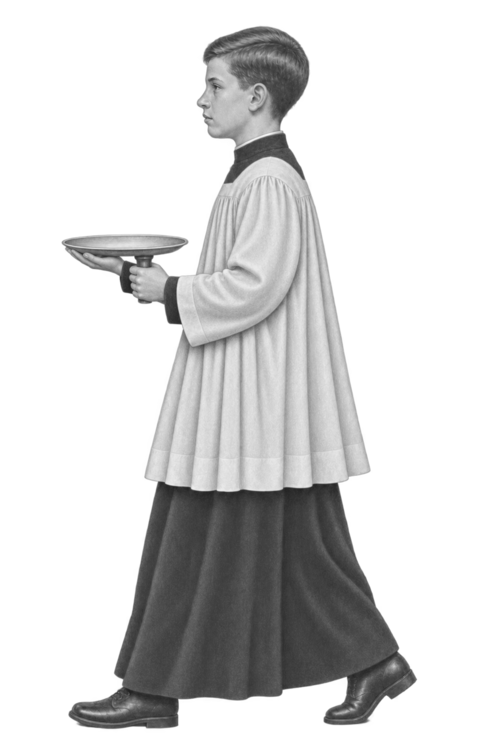
\includegraphics[height=23\ASGSceneUnit]{liturgy/roman-rite/1962/reference/altar-server-guides/shared/artwork/pencil/ASG-ART-077-server-carrying-communion-plate.png}}};
  \ASGStation{#1}{#2-2}{#3}}
\newcommand{\LMMovePlateTaken}{%
  \LMPositionScene{%
    \LMRestingLavaboTowel{93.6}{19.6}\LMRestingLavaboBasin{93.6}{19.2}
    \LMRestingCruets{97.2}{19.6}\LMRestingBell{80}{22.5}
    \LMChaliceWithPallObject{50}{43}\LMRestingVeil{70}{43}
    \LMMissalAtGospel\ASGPriest{50}{26.5}{PRIEST}
    \ASGKneelingServer{25}{18.3}{SECOND\\WAITS}
    \LMMovePlateLeft{79}{11.3}{FIRST}
    \draw[asg route] (73,6) -- (65,6);
  }{1. First leaves the credence carrying the Communion plate level in both hands; it is no longer on the table.}}
\newcommand{\LMMovePlateApproach}{%
  \LMPositionScene{%
    \LMRestingLavaboTowel{93.6}{19.6}\LMRestingLavaboBasin{93.6}{19.2}
    \LMRestingCruets{97.2}{19.6}\LMRestingBell{80}{22.5}
    \LMChaliceWithPallObject{50}{43}\LMRestingVeil{70}{43}
    \LMMissalAtGospel\LMPriestAbove{50}{26.5}
    \ASGKneelingServer{25}{18.3}{SECOND\\WAITS}
    \LMMovePlateLeft{48}{11.3}{FIRST}
  }{2. First reaches the rehearsed floor approach point, ready to join the priest's right when he comes to distribute.}}
\newcommand{\LMMovePlateCollected}{%
  \LMPositionScene{%
    \LMRestingLavaboTowel{93.6}{19.6}\LMRestingLavaboBasin{93.6}{19.2}
    \LMRestingCruets{97.2}{19.6}\LMRestingBell{80}{22.5}
    \LMUncoveredChaliceObject{44}{43}\LMRestingVeil{70}{43}
    \LMMissalAtGospel\ASGPriest{50}{26.5}{PRIEST}
    \ASGStandingServer{25}{11.3}{SECOND\\WAITS}
    \LMMovePlateRight{77}{26.5}{FIRST}
    \draw[asg route] (82,25) -- (85,21);
  }{1. After the final water and the priest's signal, First has collected the cleared plate at Epistle and turned to descend.}}
\newcommand{\LMMovePlateReturning}{%
  \LMPositionScene{%
    \LMRestingLavaboTowel{93.6}{19.6}\LMRestingLavaboBasin{93.6}{19.2}
    \LMRestingCruets{97.2}{19.6}\LMRestingBell{80}{22.5}
    \LMUncoveredChaliceObject{44}{43}\LMRestingVeil{70}{43}
    \LMMissalAtGospel\ASGPriest{50}{26.5}{PRIEST}
    \ASGStandingServer{25}{11.3}{SECOND\\WAITS}
    \LMMovePlateRight{83}{11.3}{FIRST}
    \draw[asg route] (85,6) -- (90,6);
  }{2. Back on the floor, First carries the cleared plate toward the credence; keep it level until it rests on the table.}}

